\documentclass[10pt,cours,a4paper,firamath]{nsi}
\begin{document}
\chapter{BDD partie 1}
\section{Introduction}
\subsection{BDD et SGBD}
Une \textit{base de données} (BDD) est un ensemble structuré de données ainsi que des relations logiques sur ces données.\\

Le \textit{système de gestion de bases de données} (SGBD) peut être vu comme le logiciel qui gère :
\begin{itemize}
    \item	la structuration des données ;
    \item	le stockage des données ;
    \item 	la maintenance des données ;
    \item 	la sécurité des données ;
    \item 	les accès aux données (lecture et/ou écriture) en temps réel par de multiples intervenants.
\end{itemize}


\subsection{Un peu d'histoire}
La majorité de ce que nous allons voir repose sur les travaux d'Edgar F. Codd, c'est lui qui a inventé le modèle relationnel en 1970 alors qu'il travaillait comme informaticien chez IBM.
\begin{center}
    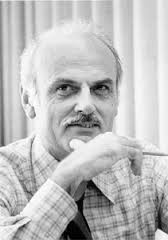
\includegraphics[width=3cm]{img/codd}
\end{center}


\subsection{Phases de conception d'une BDD}
C'est une tâche essentielle pour assurer le bon fonctionnement des applications qui vont l'utiliser.
\begin{itemize}
    \item	\textit{niveau conceptuel} : on représente la BDD à l'aide de schémas indépendamment de toute considération informatique ;
    \item	\textit{niveau logique} on adapte le schéma en tables à deux dimensions ;
    \item	\textit{niveau physique} on implémente les tables sur un SGBD.
\end{itemize}

\section{Niveau conceptuel : modèle entités-associations}
\subsection{Entités}
On commence par déterminer les types des entités qui interviennent:
\begin{itemize}
    \item	une \textit{entité} est un objet unique avec un nombre fini d'attributs ;
    \item	un (ou plusieurs) attribut(s) permet(tent) d'identifier de manière unique l'entité : on parle d'\textit{identifian}t(s) ou de clé.
\end{itemize}
\begin{center}
    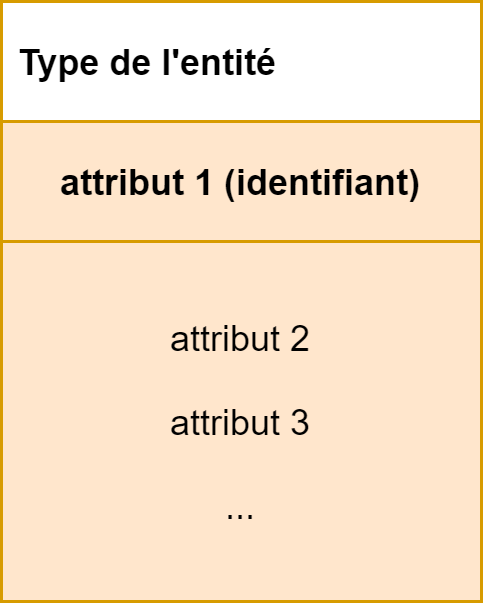
\includegraphics[width=3cm]{img/entité}
\end{center}

\begin{exemple}[ : entité-type Auteur]
    \begin{center}
        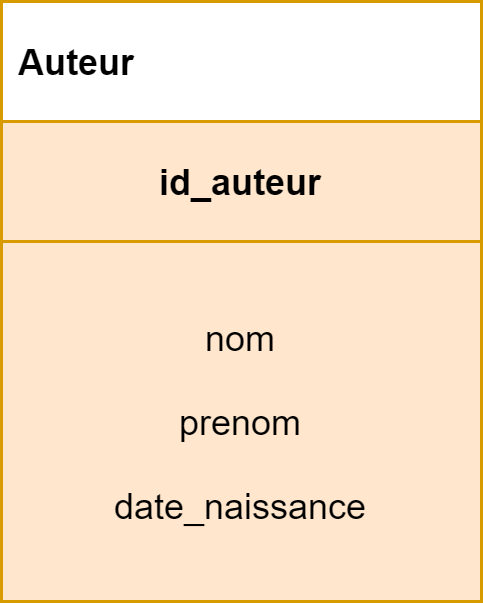
\includegraphics[width=3cm]{img/auteur}
    \end{center}
\end{exemple}
\subsection{Occurrences}

Une entité-type a en général plusieurs occurrences, appelées entités.\\

\begin{center}
    \tabstyle[UGLiBlue]
    \begin{tabular}{cccc}
        \hline
        
        \ccell{id\_auteur } & \ccell{nom} & \ccell{prenom} & \ccell{date\_naissance} \\\hline
        00000001            & Dupond      & Marie          & 23/08/1982              \\
        12345678            & Martin      & Luce           & 13/05/1963              \\
        98765432            & Leblanc     & Jean           & 18/11/1974              \\
        \hline
    \end{tabular}
\end{center}
\begin{remarque}
    Par souci de simplicité, on parlera d'entité à la fois pour désigner l'entité-type et chacune de ses occurrences.
\end{remarque}

\subsection{Entité Pays}
Voici une autre entité entrant en jeu dans la BDD :
\begin{center}
    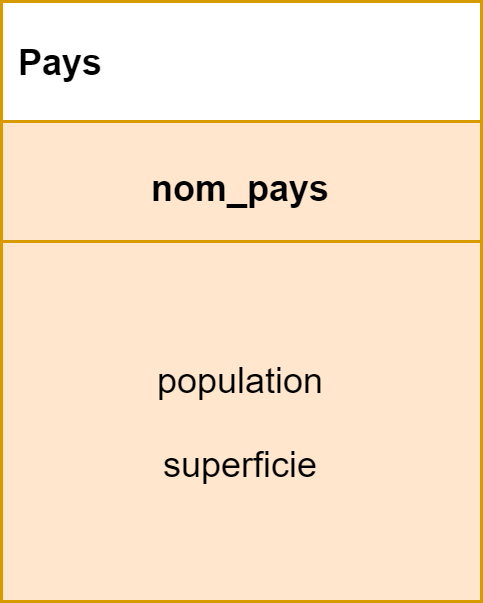
\includegraphics[width=3cm]{img/pays}
\end{center}


\subsection{Associations}
Elles définissent des \textit{liens sémantiques} (des liens de sens)	 que les simples entités ne suffisent pas à définir.\\

Une association comporte :
\begin{itemize}
    \item	un nom;
    \item 	un lien entre 2 relations ;
    \item	deux cardinalités qui sont représentées sur les extrémités du lien ;
    \item 	parfois elle peut comporter un ou des attributs.
\end{itemize}

\begin{exemple}[]
    \begin{center}
        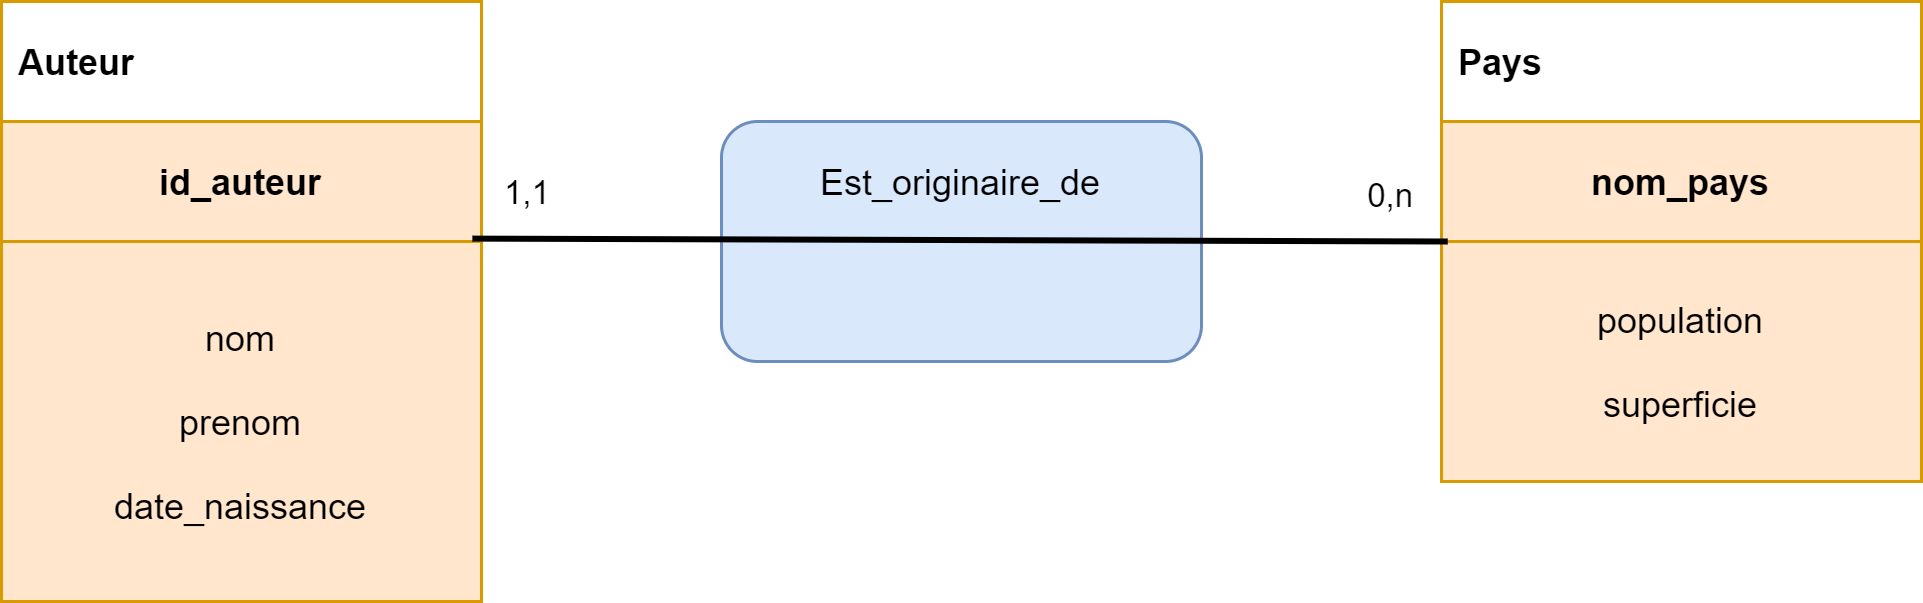
\includegraphics[width=11cm]{img/schema_1}
    \end{center}
    Une cardinalité est un couple d'entiers « de type $\min, \max$» :
    \begin{itemize}
        \item	la cardinalité 1,1 signifie qu'un auteur peut être lié au minimum à 1 pays, et au maximum à 1 pays (donc à un pays et un seul) ;
        \item	la cardinalité 0,n signifie qu'un pays peut être lié au minimum à aucun auteur et au maximum plusieurs auteurs.
    \end{itemize}
\end{exemple}


\subsection{Un schéma abouti}
\begin{center}
    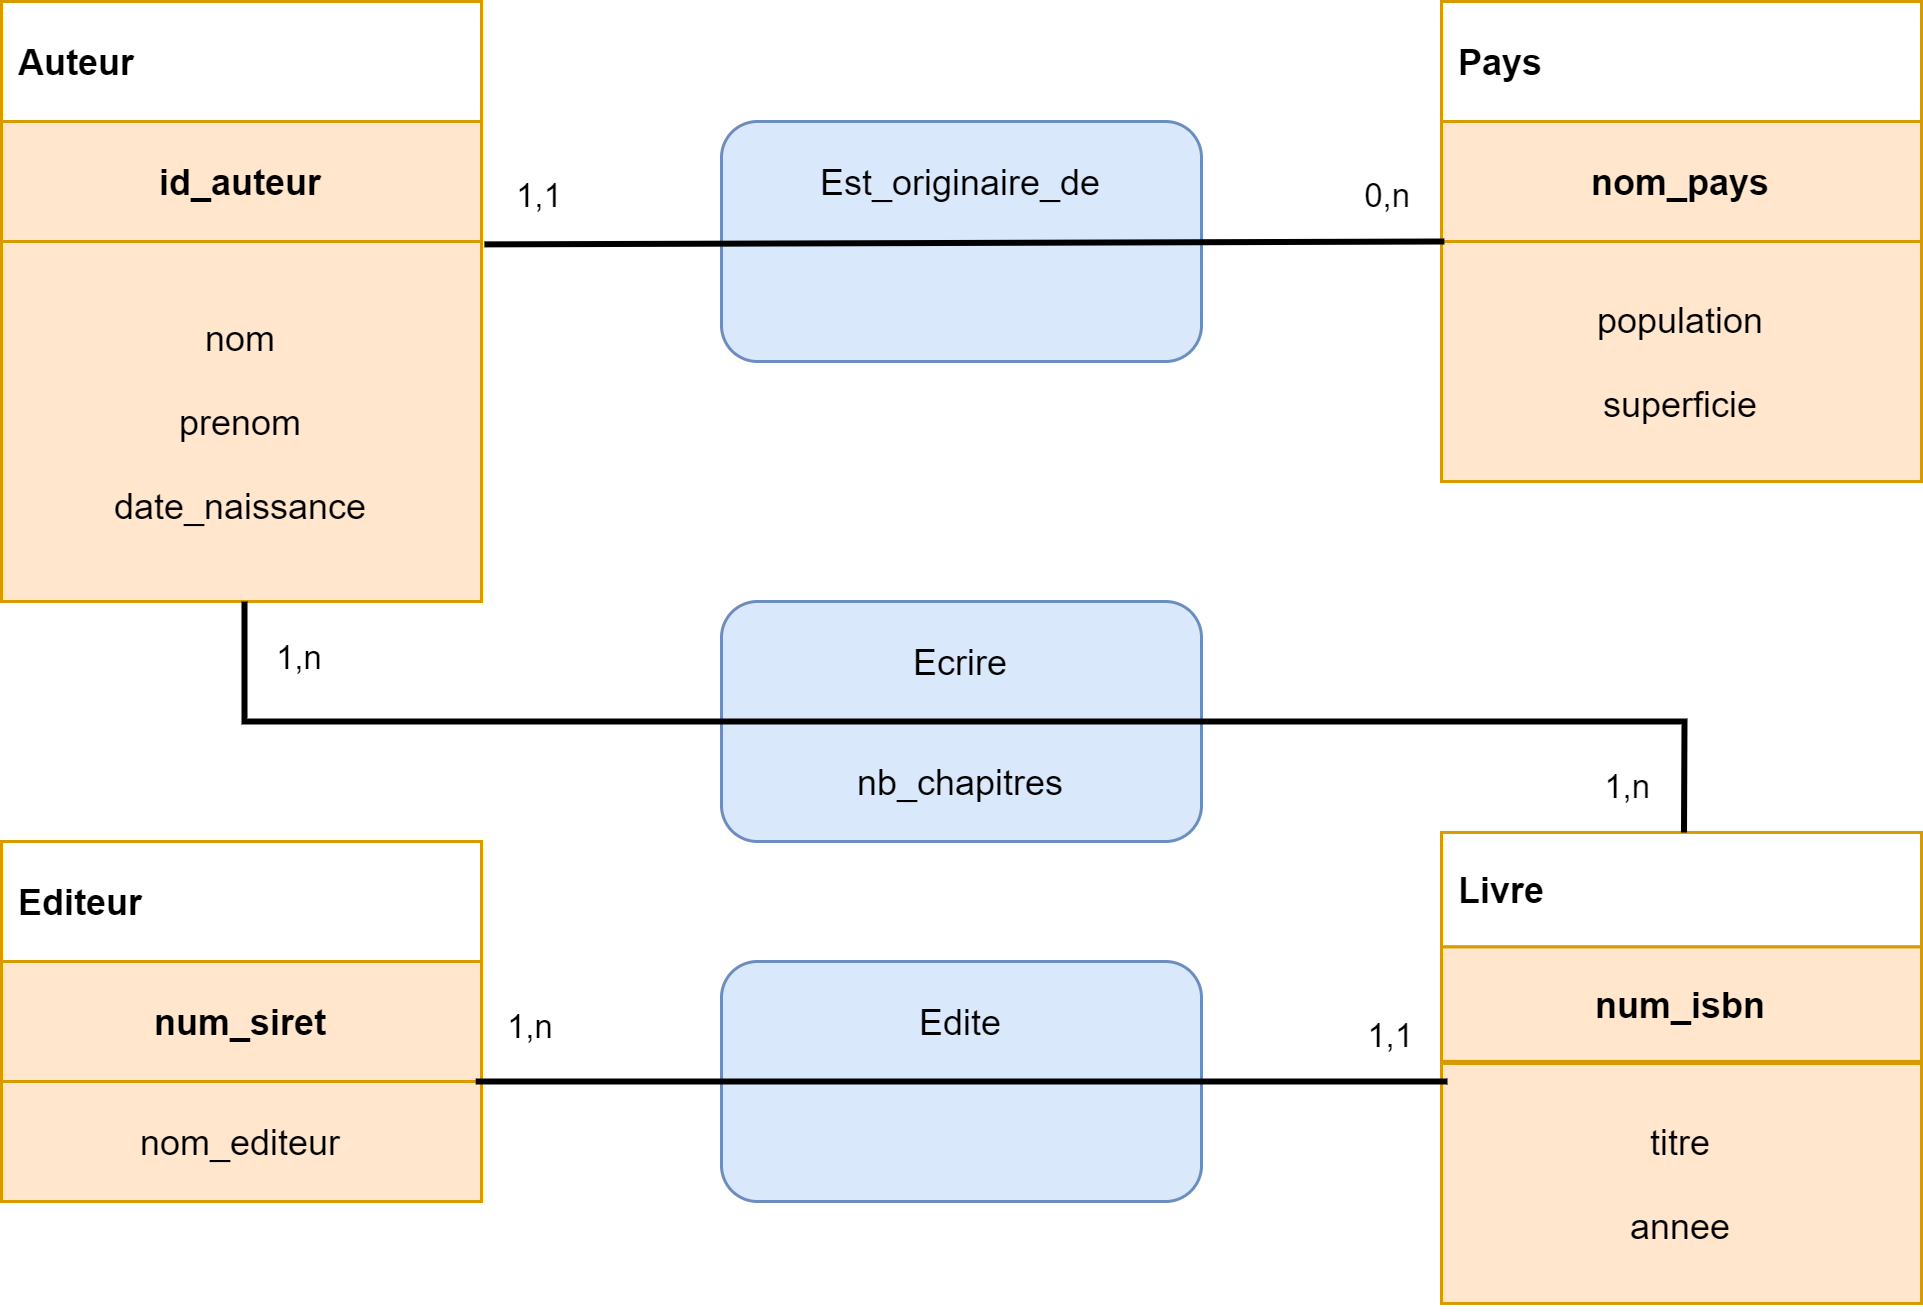
\includegraphics[width=11cm]{img/schema_2}
\end{center}

\subsection{Non-unicité des schémas}
Le schéma précédent s'appelle un modèle conceptuel des données (MCD).\\
On peut modéliser une situation avec plusieurs MCD, chacun d'entre eux ont leurs avantages et leurs inconvénients.

\section{Exercices}

\begin{exercice}[]
    \begin{center}
        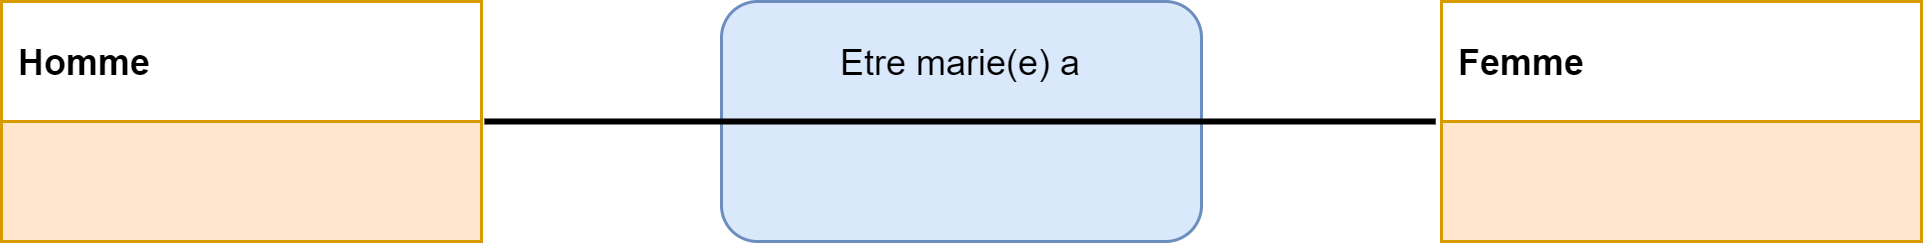
\includegraphics[width=12cm]{img/ex1}
    \end{center}
    Préciser les cardinalités de l'association \textit{Etre marie(e) a} :
    \begin{itemize}
        \item 	dans une société monogame ;
        \item 	dans une société dans laquelle les femmes ont le droit d'être polygames.
    \end{itemize}
\end{exercice}

\begin{exercice}[]
    \begin{center}
        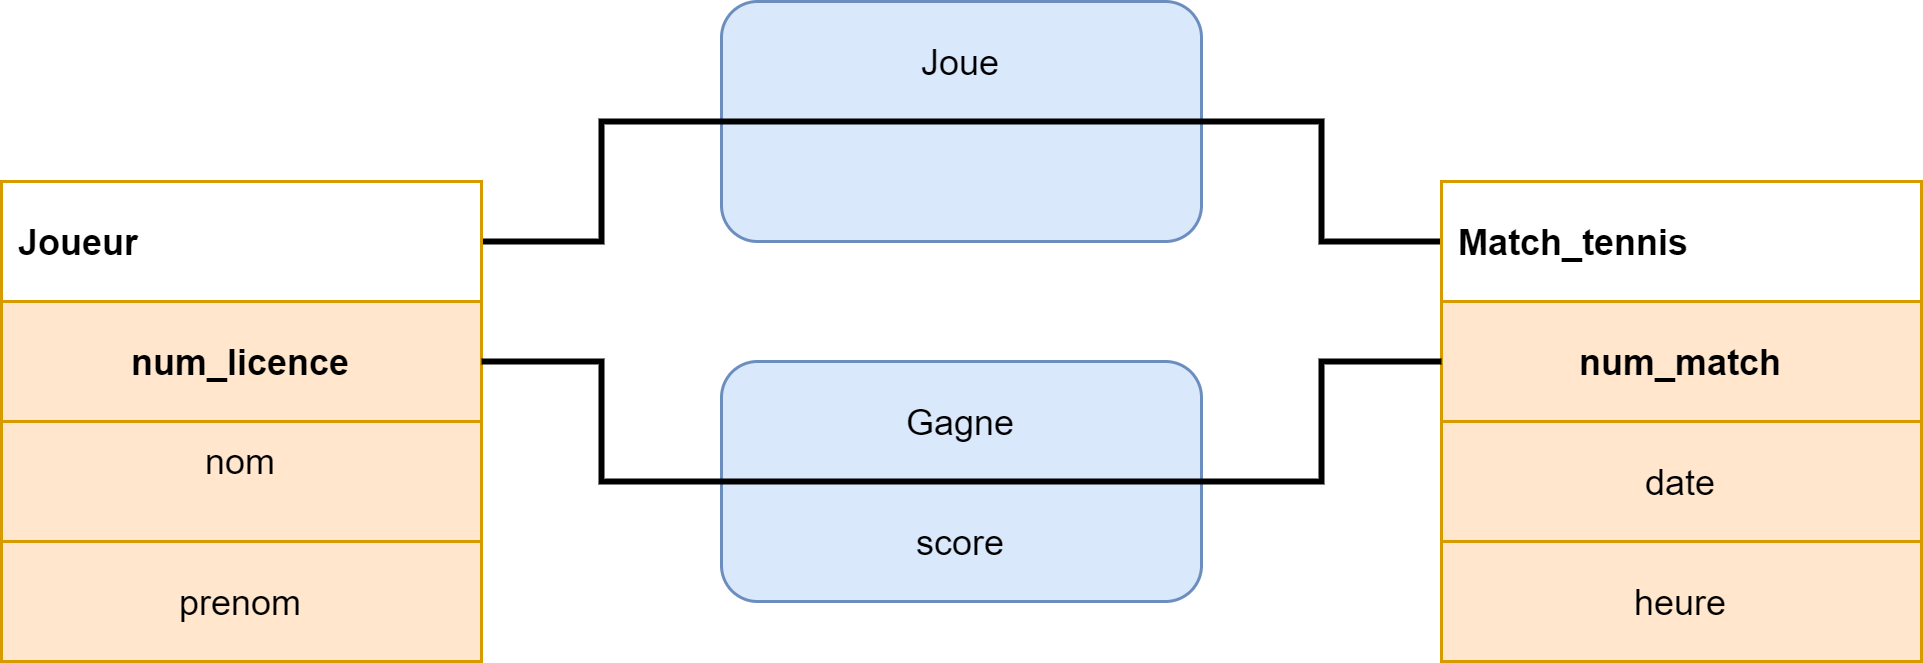
\includegraphics[width=12cm]{img/ex2}
    \end{center}
    Préciser les cardinalités des associations.
\end{exercice}
\newpage

\begin{exercice}[]
    \begin{center}
        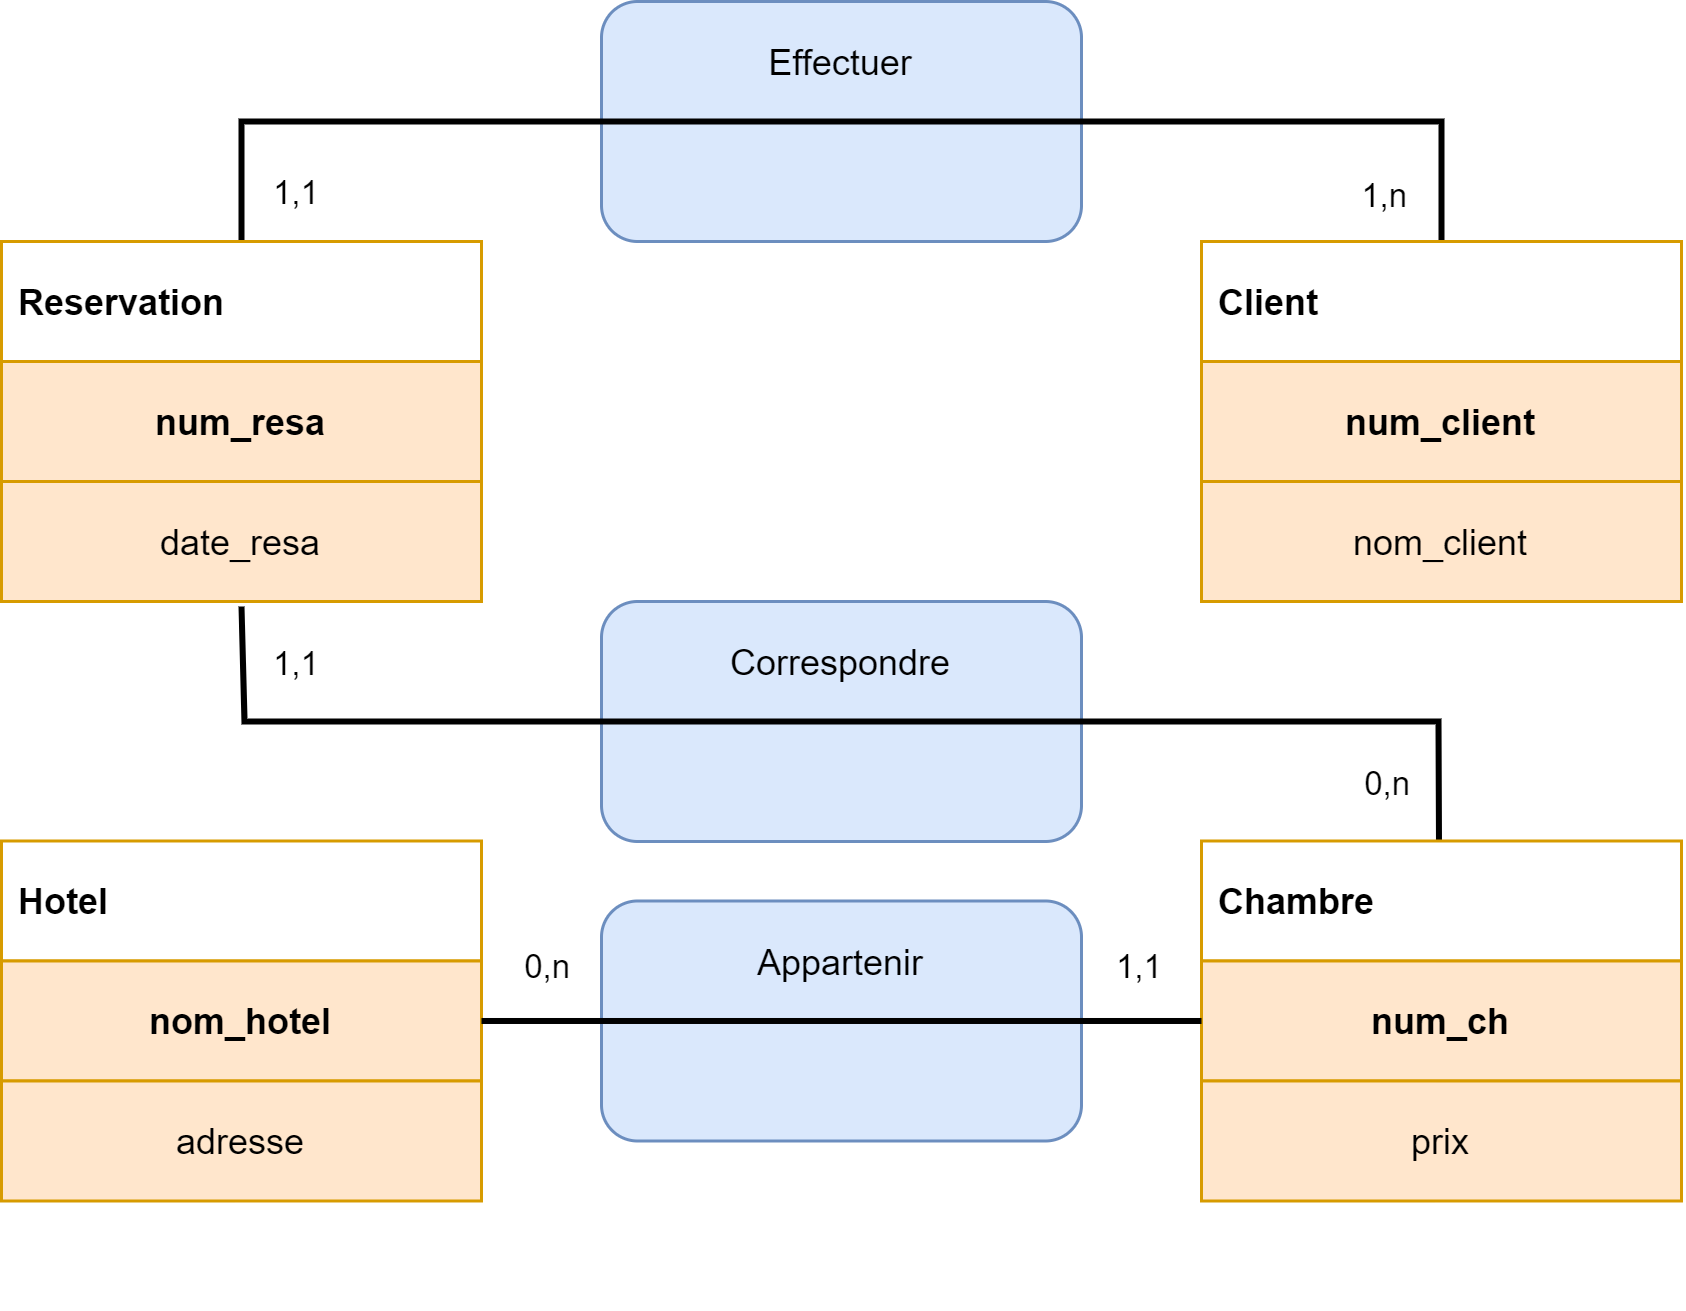
\includegraphics[width=12cm]{img/ex_hotel}
    \end{center}
    Dans ce modèle
    \begin{enumerate}
        \item 	Peut-on avoir des clients homonymes ?
        \item 	Un client peut-il réserver plusieurs chambres à une même date ?
        \item 	Est-il possible de réserver une chambre plusieurs jours d'affilée ?
        \item 	Peut-on savoir si une chambre est libre à une date donnée ?
        \item 	Peut-on réserver la même chambre plusieurs fois à la même date ?
    \end{enumerate}
\end{exercice}
\newpage
\begin{exercice}[]
    \begin{center}
        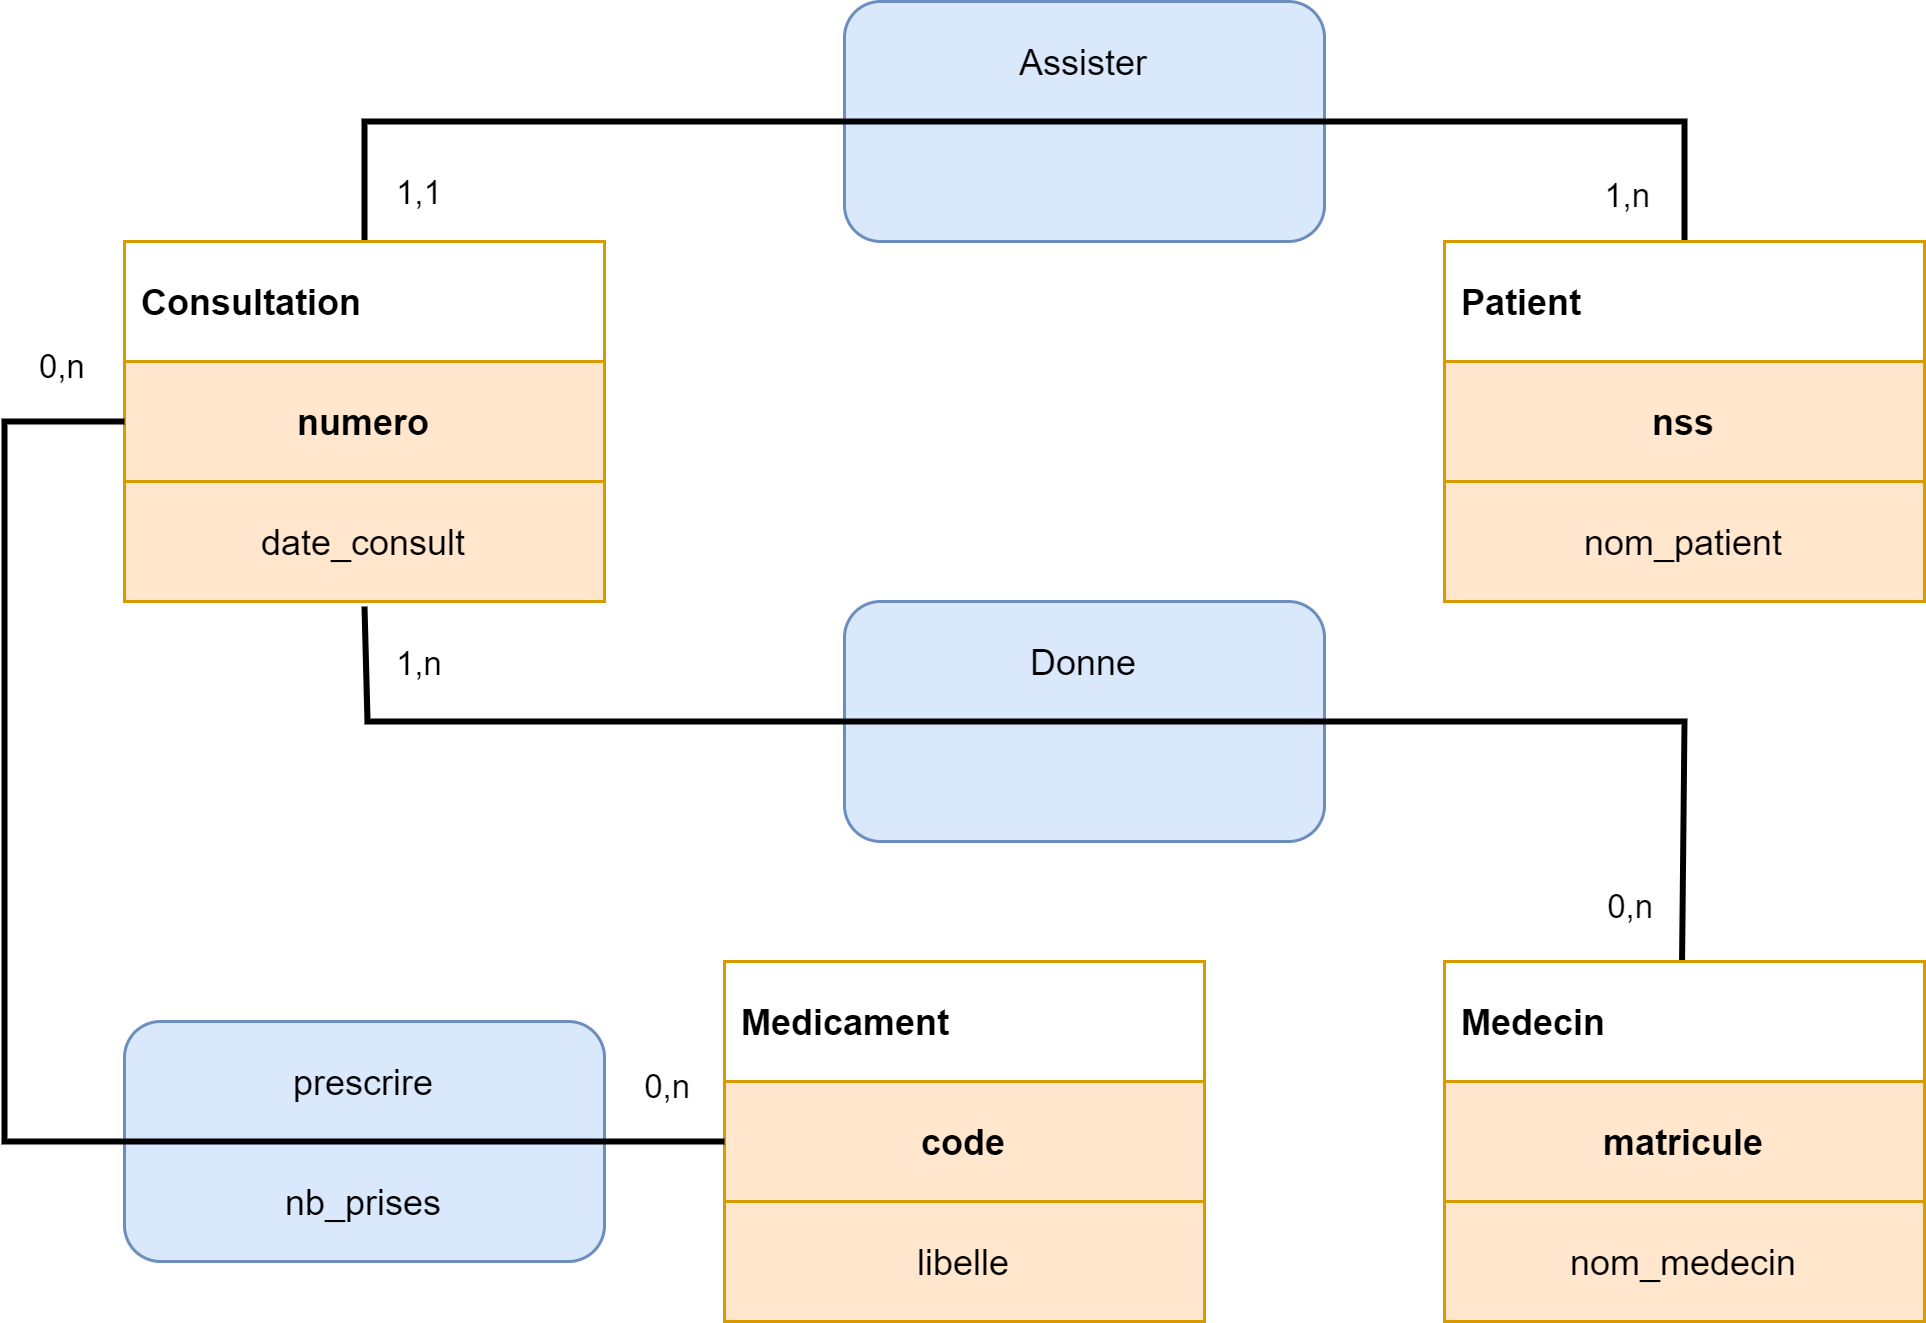
\includegraphics[width=12cm]{img/ex_consultation}
    \end{center}
    Dans ce modèle
    \begin{enumerate}
        \item 	Un patient peut-il assister à plusieurs consultations ?
        \item   Deux patients peuvent-ils assister à la même consultation ?
        \item   Deux consultations peuvent-elles avoir lieu le même jour ?
        \item 	Un médecin peut-il recevoir plusieurs patients lors d'une même consultation ?
        \item   Plusieurs médecins peuvent-ils assister à la même consultation ?
        \item   Une consultation entraîne-t-elle toujours une prescription ?
        \item 	Peut-on prescrire plusieurs médicaments lors d'une même consultation ?
        \item   Deux médecins différents peuvent-ils prescrire le même médicament ?
        \item   \'Etant donné un médicament prescrit, peut-on toujours connaître le médecin qui l'a prescrit ?
              
    \end{enumerate}
\end{exercice}


\begin{exercice}[]
    Une entreprise est identifiée par son nom.\\
    Dans cette entreprise, un département est identifié par un nom et caractérisé par une localisation.\\
    Un employé est caractérisé par un numéro, son nom, son grade et le département dans lequel il travaille.\\
    Le numéro d'un employé est unique dans un département mais pas dans l'entreprise.\\
    Donner le MCD, en précisant les attributs.\\
    
    \textit{Indication : « caractérisé» fait référence à un attribut, « identifié» à un identifiant.}
\end{exercice}

\begin{exercice}[]
    \begin{center}
        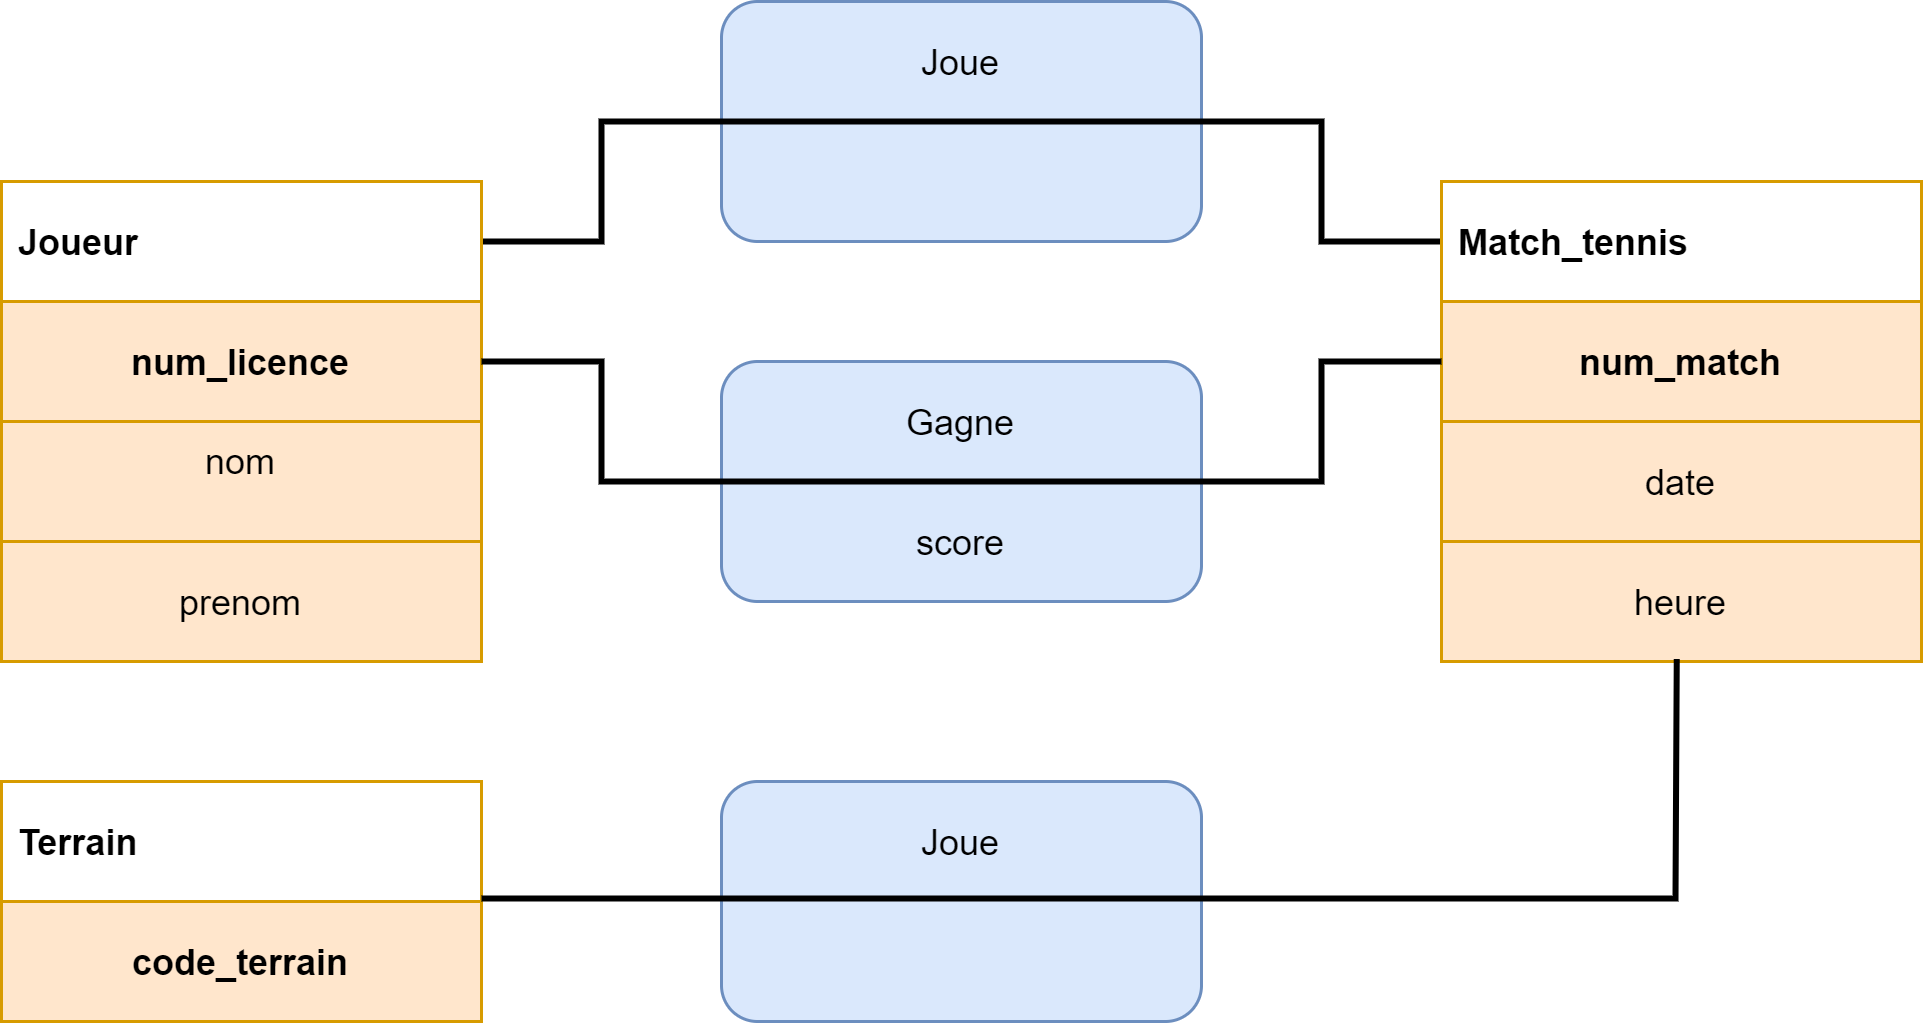
\includegraphics[width=12cm]{img/ex3}
    \end{center}
    \begin{enumerate}
        \item 	Reprendre les cardinalités du précédent MCD sur le tennis et préciser celle de \textit{Joue}.
        \item 	Selon ce modèle peut-on jouer des matchs de double ?
        \item 	Un joueur peut-il gagner un match sans y avoir participé ?
        \item 	Peut-il y avoir 2 matchs sur le même terrain à la même heure ?
        \item 	Connaissant un joueur, peut-on savoir sur quel(s) terrain(s) il a joué ?
    \end{enumerate}
\end{exercice}

\begin{exercice}[]
    On considère une médiathèque contenant des ouvrages pouvant être empruntés.\\
    Un ouvrage est caractérisé par un numéro unique, un titre, un auteur et un éditeur. En outre, on décrit un ouvrage par un certain nombre de mots-clés qui indiquent les sujets qui y sont traités.\\
    La médiathèque dispose d'un ou plusieurs exemplaires de chaque ouvrage, L'exemplaire est identifié par un numéro et caractérisé par sa position dans les rayonnages et sa date d'achat.
    Un exemplaire peut être emprunté par un emprunteur. Ces derniers sont identifiés par un numéro d'emprunteur et possèdent un nom et une adresse.\\
    
    Donner le MCD.
\end{exercice}

\chapter{BDD partie 2}


\section{Niveau logique : modèle relationnel}
\subsection{Principe}
On adapte un MCD en tables à deux dimensions.\\
On décide du type des attributs.\\
Pour l'instant, on peut utiliser des types génériques, qui sont susceptibles de varier légèrement d'un SGBD à un autre :
\begin{itemize}
	\item	\mintinline{sql}{INTEGER} pour les entiers;
	\item	\mintinline{sql}{FLOAT} ou \mintinline{sql}{REAL} pour les nombres en virgule flottante;
	\item	\mintinline{sql}{VARCHAR(taille)} ou \mintinline{sql}{TEXT} pour les chaînes de caractères de taille fixe ou illimitée;
	\item 	\mintinline{sql}{BIT} pour les booléens;
	\item 	\mintinline{sql}{DATE} et \mintinline{sql}{TIME} pour les heures et les dates;
\end{itemize}



\subsection{Transformer une entité en relation}
On va transformer chaque entité du MCD en \textit{relation} :
\begin{center}
	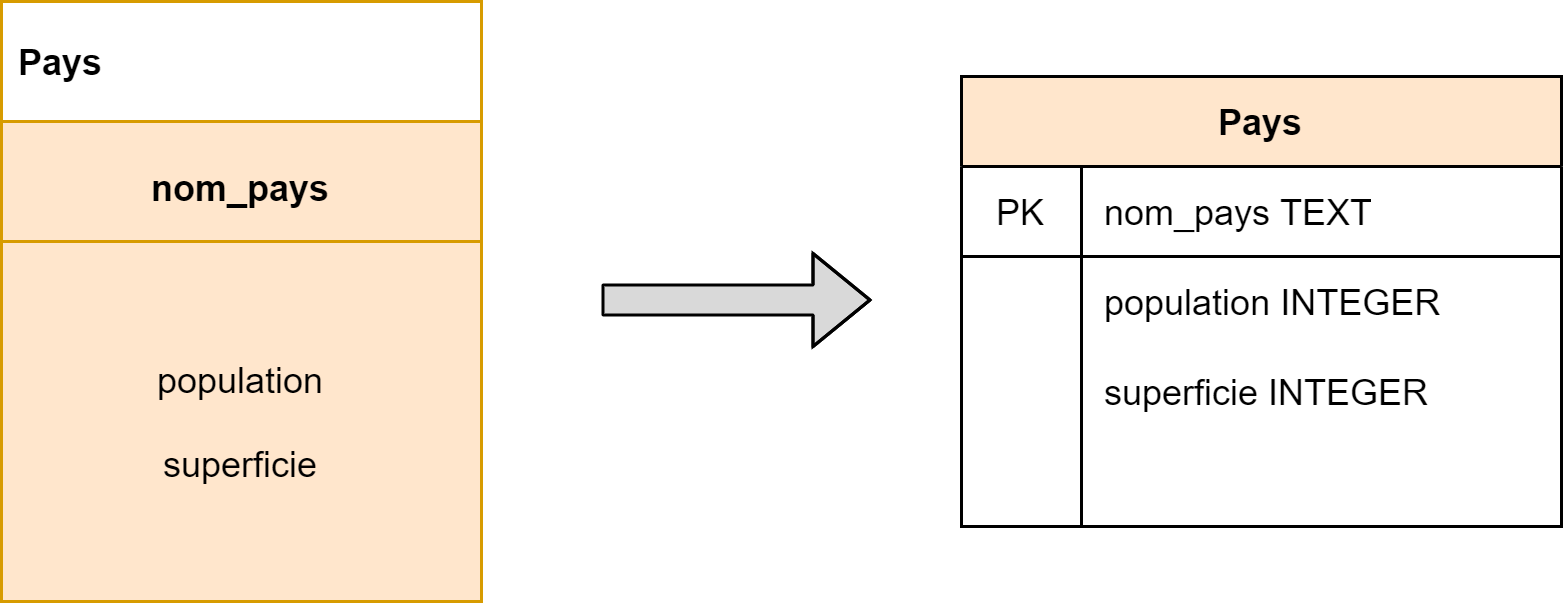
\includegraphics[width=7cm]{img/entite_vers_relation}
\end{center}
On indique les types de chaque attribut de la relation.

Le ou les identifiants de l'entité sont appelés des \textit{clés primaires} pour la relation : « PK» est l'abréviation de \mintinline{sql}{PRIMARY KEY}.\\
Le nom de la relation est noté en gras, la clé primaire soulignée.\\

\textbf{Pays}(\uline{nom\_pays TEXT}, population INTEGER, superficie INTEGER)\\




\subsubsection{Transformer une association en relation : cas (0,1) ou (1,1)}
\textit{Quand la relation possède une cardinalité valant (0,1) ou (1,1)}
\begin{center}
	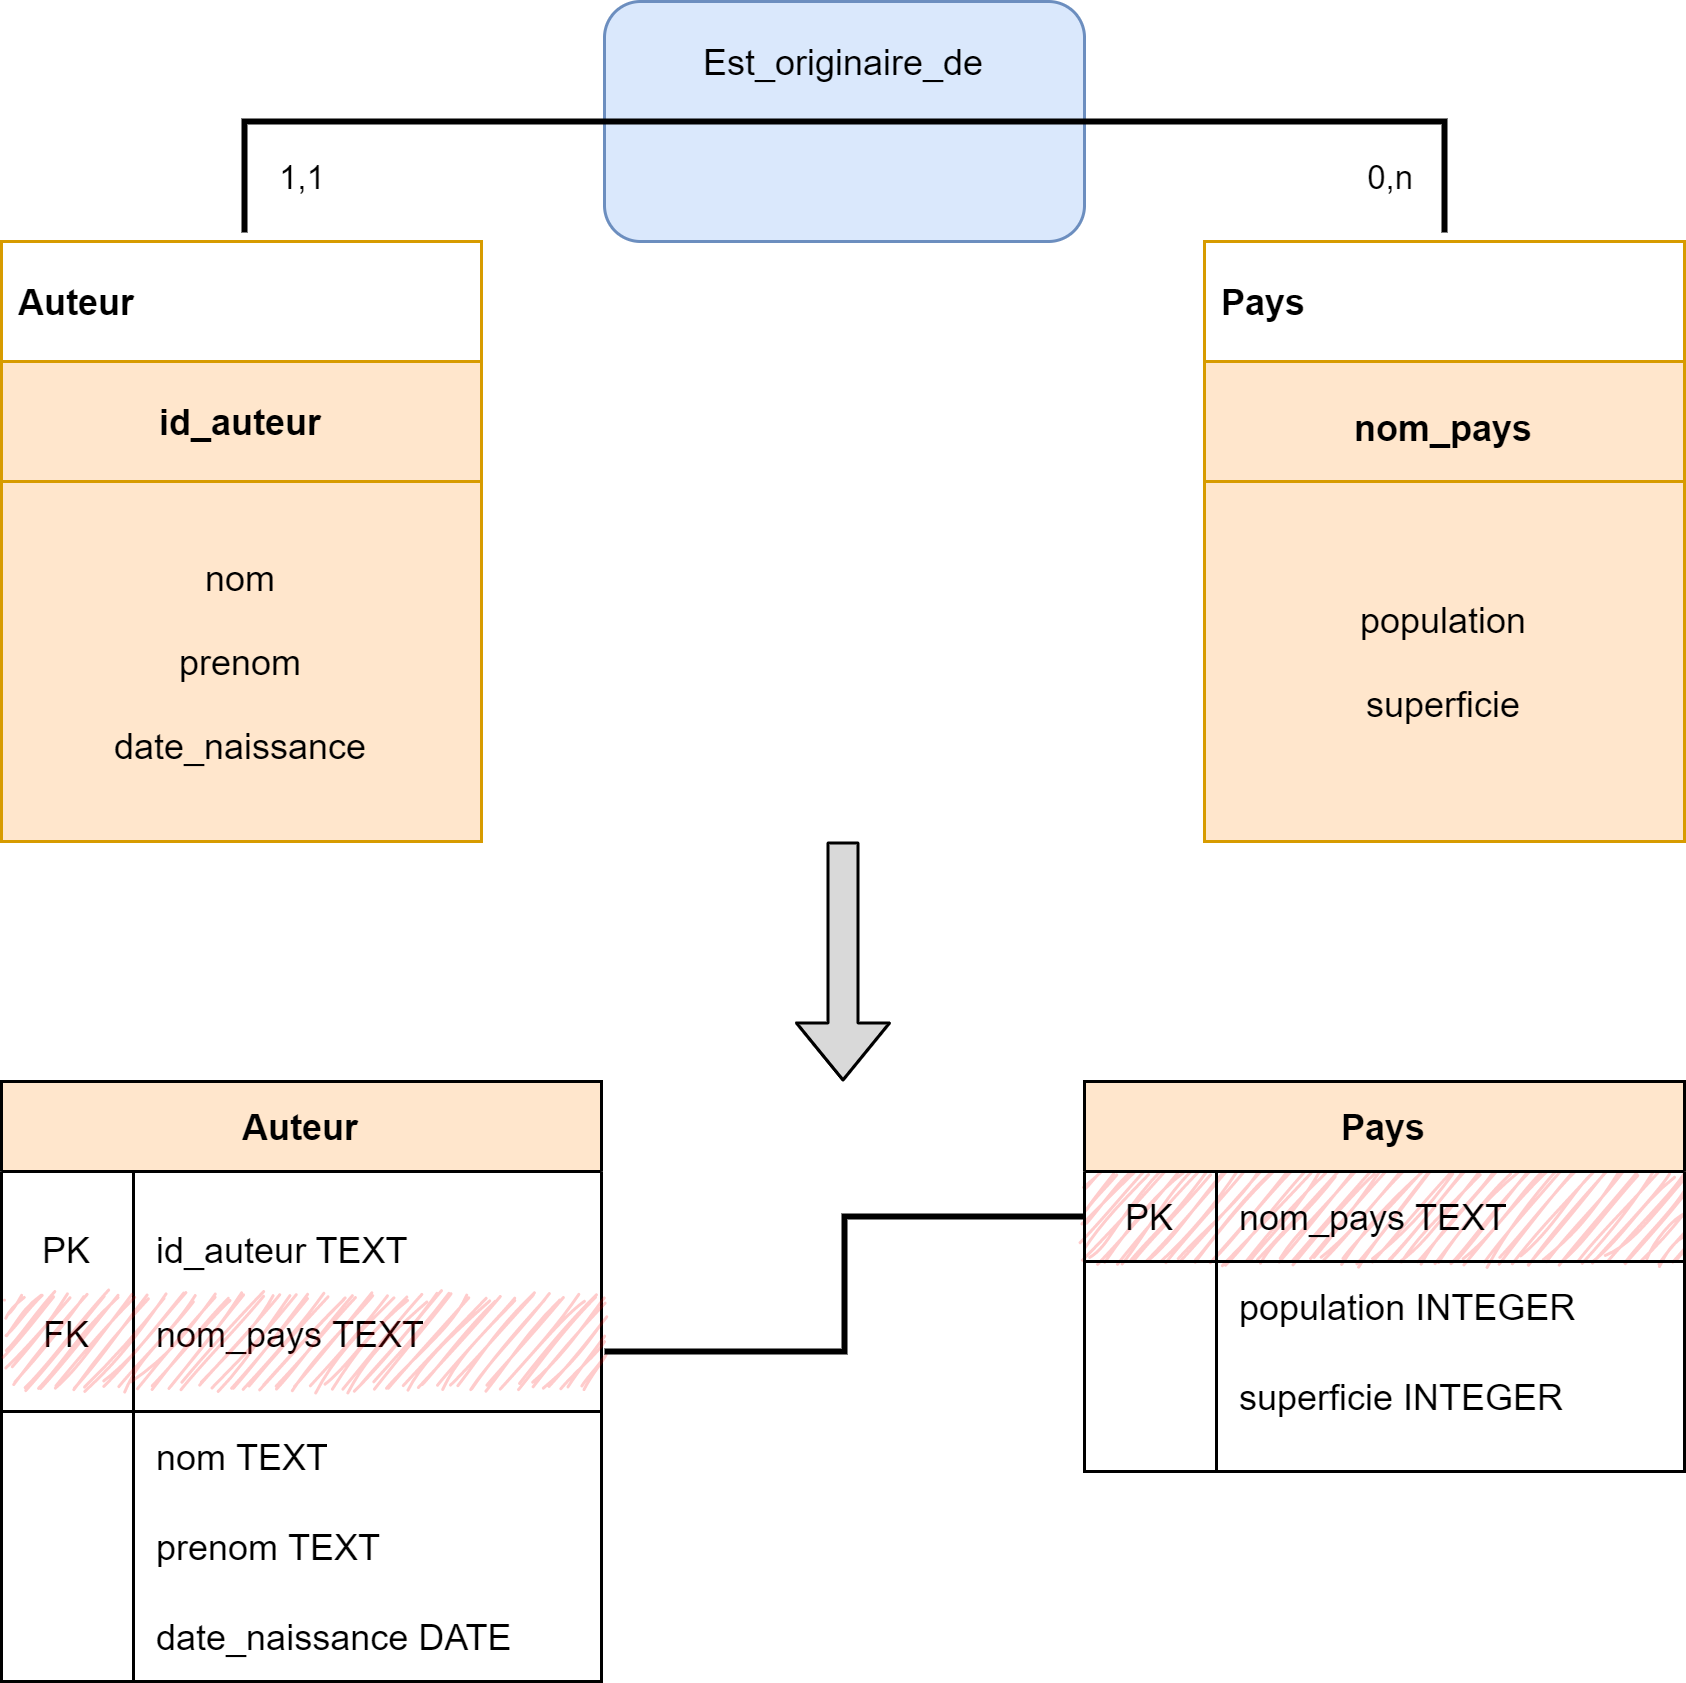
\includegraphics[width=7cm]{img/association_vers_relation_1}
\end{center}

Puisqu'un auteur vient d'un pays et un seul, on ajoute un attribut nom\_pays à la relation \textbf{Auteur}.

On précise que cet attribut est \textit{nécessairement} l'un des attributs nom de la relation \textbf{Pays} en ajoutant « FK»  dans le tableau , qui est l'abréviation de \mintinline{sql}{FOREIGN KEY}.

On dit que nom\_pays est une \textit{clé étrangère}, qui \textit{fait référence} à l'attribut nom de la relation \textbf{Pays}.

La clé étrangère est soulignée en traits discontinus.\\



\textbf{Pays}(\uline{nom\_pays TEXT }, population INTEGER, superficie INTEGER)\\

\textbf{Auteur}(\uline{id\_auteur INTEGER}, \dashuline{nom\_pays TEXT} , nom TEXT, prenom TEXTE, date\_naissance DATE)


\subsubsection{Transformer une association en relation : autre cas}
\textit{Quand la relation ne possède pas de cardinalité valant (0,1) ou (1,1)}
\begin{center}
	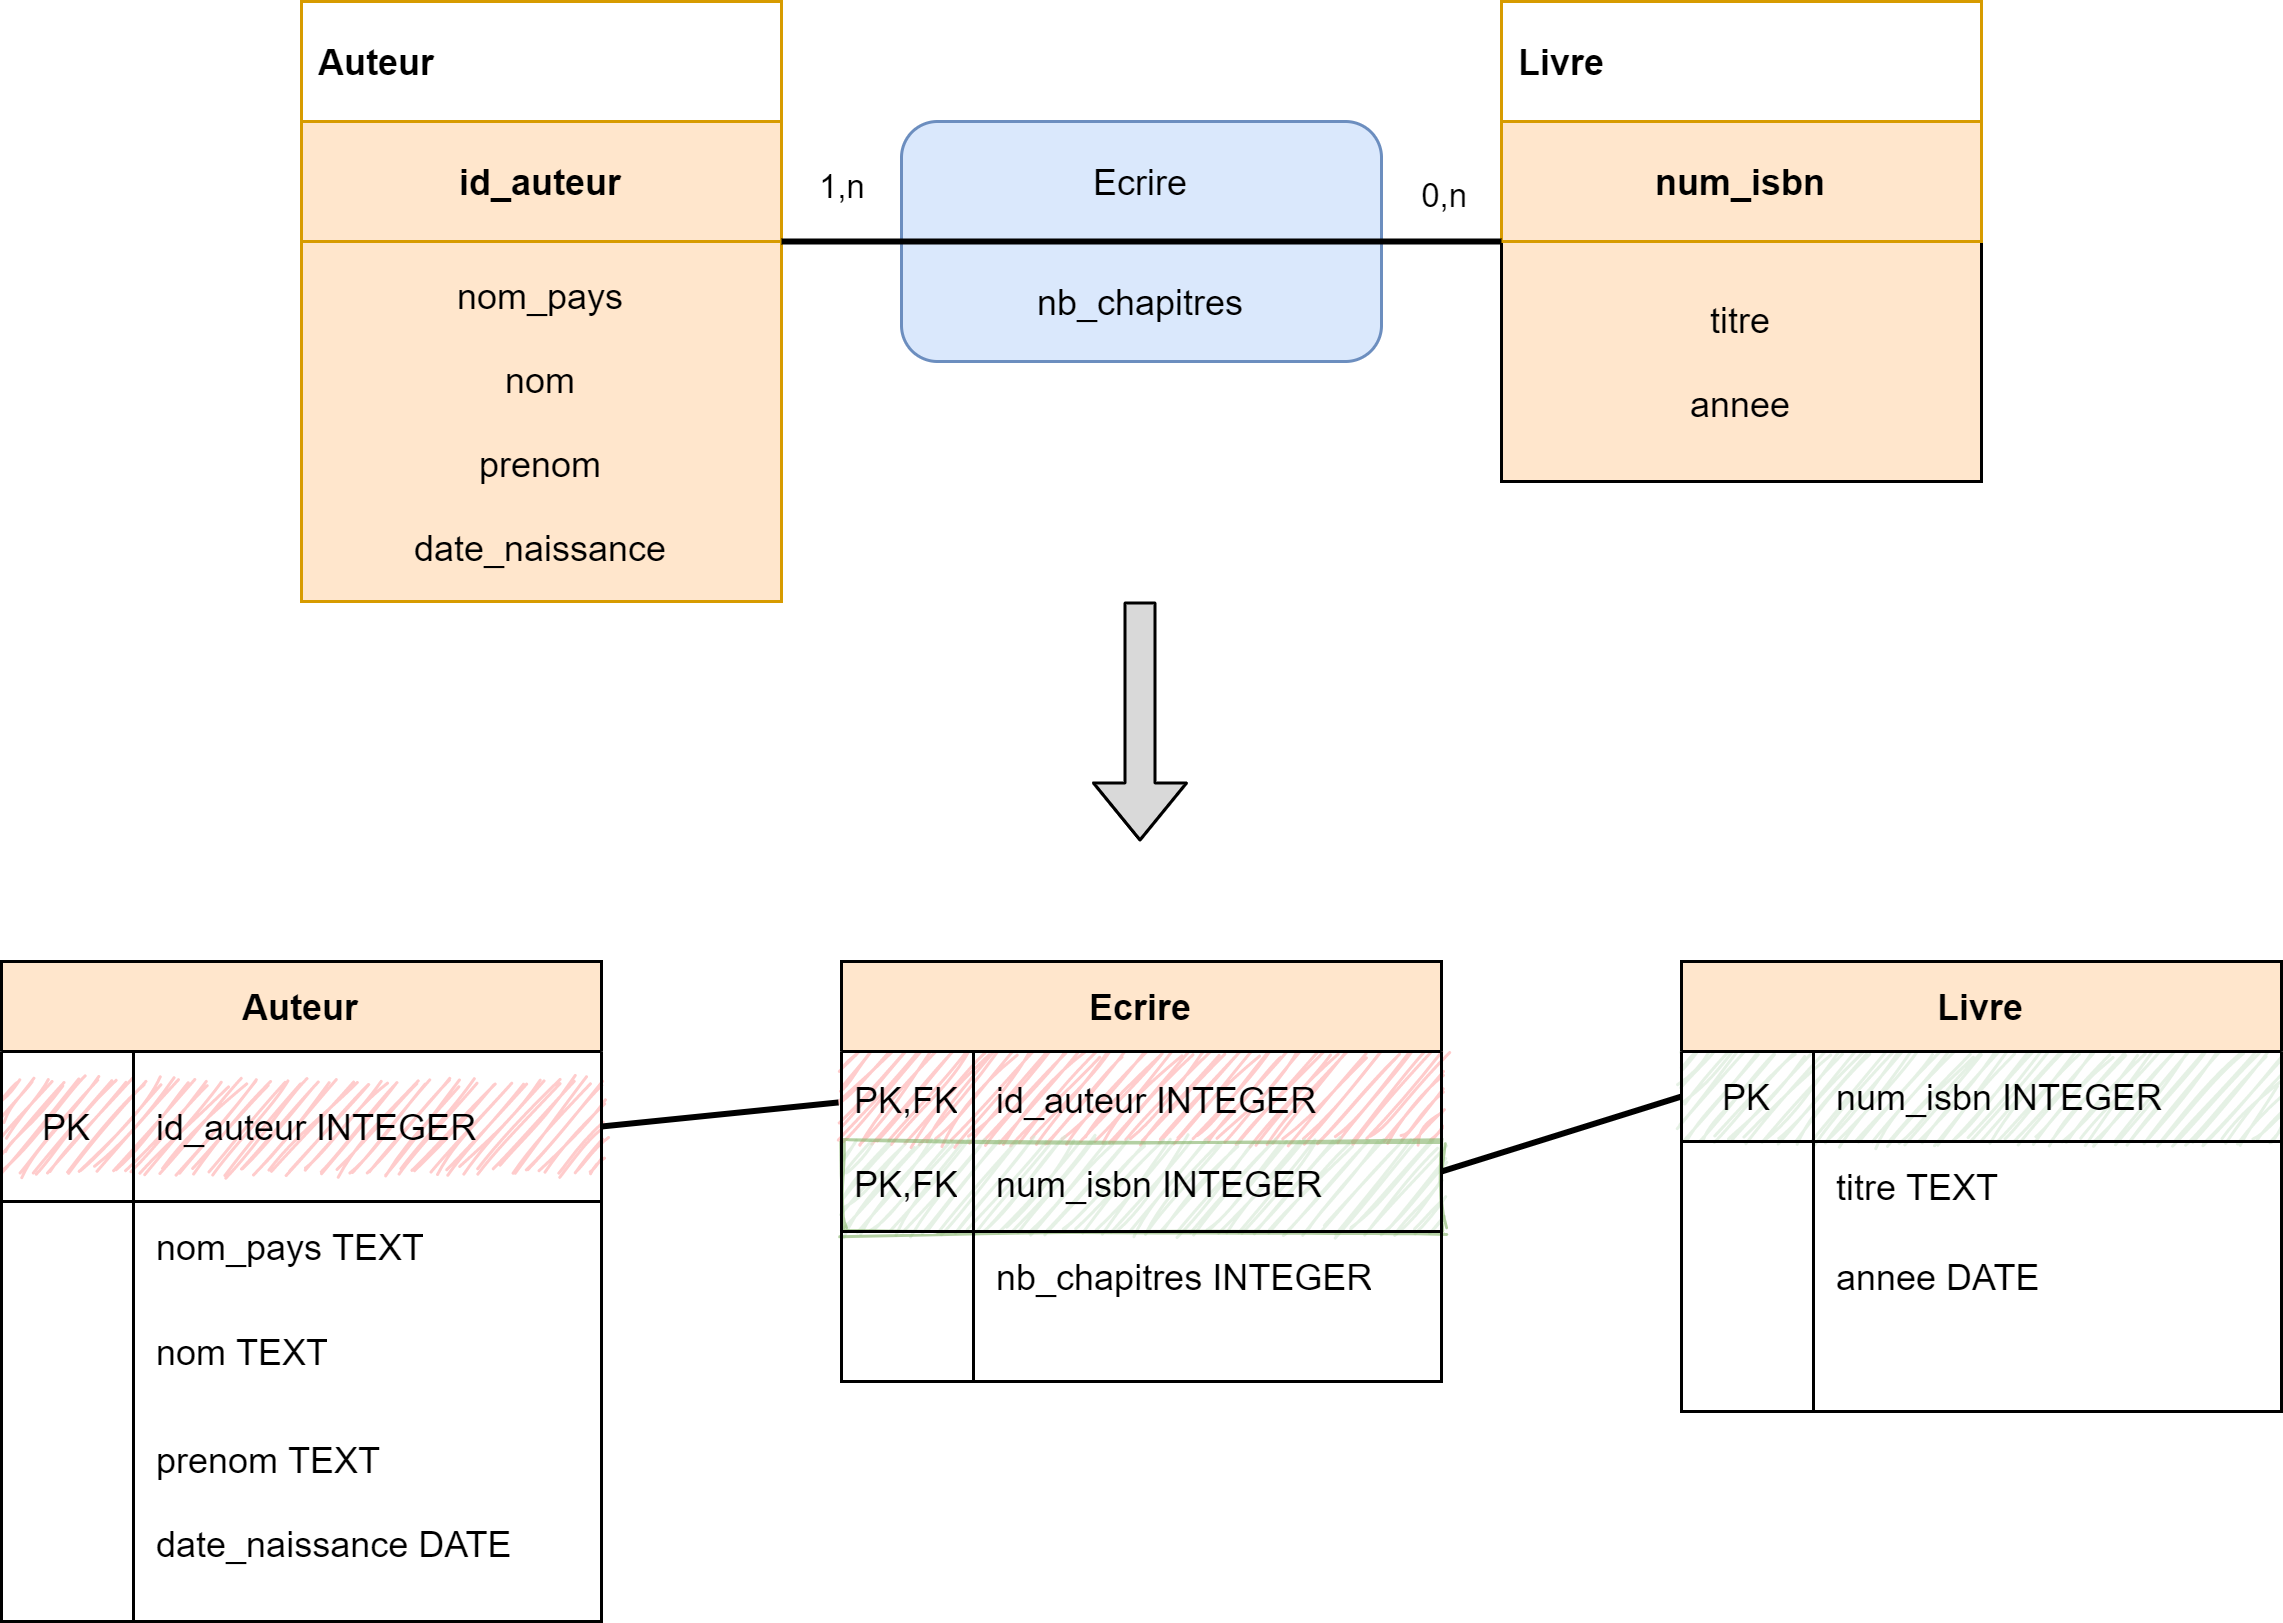
\includegraphics[width=8cm]{img/association_vers_relation_2}
\end{center}

Dans ce cas on fabrique une nouvelle relation :
\begin{itemize}
	\item on considère les clés primaires des relations issues des entités concernées par l'association;
	\item on fabrique une \textit{nouvelle relation} avec comme clé primaire ce couple de de clés primaires;
	\item ces clés primaires sont également des \textit{clés étrangères};
	\item on ajoute si besoin est d'autres attributs spécifiques à l'association.
\end{itemize}
On va noter cela

\textbf{Ecrire}(\uline{\dashuline{id\_auteur INTEGER, num\_isbn INTEGER}}, nb\_chapitres INTEGER)\\

\subsection{Modèle complet}


\textbf{Pays}(\uline{nom\_pays TEXT }, population INTEGER, superficie INTEGER)\\

\textbf{Livre}(\uline{num\_isbn INTEGER} , titre TEXT, annee DATE)\\

{\scriptsize\textbf{Auteur}(\uline{id\_auteur INTEGER}, \dashuline{nom\_pays TEXT} , nom TEXT, prenom TEXTE, date\_naissance DATE)\\}

\textbf{Ecrire}(\uline{\dashuline{ id\_auteur INTEGER, num\_isbn INTEGER}}, nb\_chapitres INTEGER)\\


\begin{remarque}[]
	Lorsqu'on modélise une BDD, on n'a pas toujours besoin de passer par le MCD pour établir le modèle relationnel : on peut parfois le faire directement.
\end{remarque}

\begin{encadrecolore}{Bilan}{UGLiBlue}
	Lorsqu'on établit un modèle relationnel (à partir d'un MCD ou directement) on définit des relations qui symbolisent des entités ou des associations.
	
	On définit aussi les \textit{contraintes} de la BDD :
	\begin{itemize}
		\item	\textit{Contraintes de domaines} : c'est essentiellement définir le type des attributs des relations;
		\item	\textit{Contraintes d'entité} : c'est déterminer des clés primaires pour garantir l'unicité de chaque élément d'une relation;
		\item 	\textit{Contraintes de référence} : c'est déterminer les clés étrangères dans les relations;
		\item 	\textit{Contraintes utilisateur} : ce sont des contraintes sur les valeurs des attributs qui garantissent leur cohérence.
	\end{itemize}
\end{encadrecolore}

\subsection{Contraintes}
Ces contraintes vont garantir la cohérence logique de la future base de données
\begin{itemize}
	\item	à tout instant;
	\item	dans le cas d'une mise à jour des données (insertion ou suppression d'éléments de la relation).
\end{itemize}

\begin{exemple}[ de contraintes utilisateur]
	Dans la relation \textbf{Pays}(\uline{nom\_pays TEXT }, population INTEGER, superficie INTEGER)\\
	
	On peut rajouter les contraintes utilisateurs suivantes :
	\begin{itemize}
		\item 	population > 0;
		\item 	superficie > 0.
	\end{itemize}
	De même dans \textbf{Auteur} et \textbf{Livre} on peut décider que les dates doivent être postérieures à une date donnée.	
\end{exemple}
\section{Exercices}

\begin{exercice}[]
	Reprendre le MCD de l'exercice 3 du chapitre « BBD partie 1» (\textbf{Hotel Reservation Client Chambre}) et donner le modèle relationnel
	\begin{itemize}
		\item	sous la forme d'un schéma;
		\item	sous forme écrite
	\end{itemize}
\end{exercice}

\begin{exercice}[]
	Reprendre le MCD de l'exercice 4 du chapitre « BBD partie 1» (\textbf{Consultation Patient Medicament Medecin}) et donner le modèle relationnel
	\begin{itemize}
		\item	sous la forme d'un schéma;
		\item	sous forme écrite
	\end{itemize}
\end{exercice}

\begin{exercice}[]
	Donner la modélisation relationnelle d'un bulletin scolaire. Elle doit permettre de représenter
	\begin{enumerate}
		\item 	des élèves possédants un numéro d'identifiant alphanumérique unique;
		\item 	des matières, qui grâce à la dernière réforme du lycée, varient d'un élève à l'autre;
		\item 	au plus une note sur 20 par matière.
	\end{enumerate}
\end{exercice}

\begin{exercice}[]
	On modélise un annuaire téléphonique de la manière suivante :\\
	
	\texttt{\textbf{Annuaire}(nom TEXT, prenom TEXT, \uline{tel TEXT})}\\
	
	Dire si les ensembles suivants sont valides pour cette modélisation.
	\begin{enumerate}
		\item 	\texttt{\{\}}
		\item 	\texttt{\{('titi', 'toto', '0123456789')\}}
		\item 	\texttt{\{('titi', 'toto', '0123456789'),('tata', 'tutu', '0123456789')\}}
		\item 	\texttt{\{('titi', 'toto', '0123456789'),('titi', 'toto', '9876543210')\}}
		\item 	\texttt{\{('titi', 'toto', '0123456789'),('tata', 'tutu')\}}
		\item 	\texttt{\{('titi', 'toto', 0123456789)\}}
	\end{enumerate}
\end{exercice}

\begin{exercice}[]
	\begin{enumerate}
		\item 	Proposer une modélisation des départements français. On veut pourvoir stocker le nom, le code, le chef-lieu et la liste de tous les départements voisins.\\
		      Attention les codes de départements ne sont pas tous des nombres : 2A et 2B pour la Corse et les départements d'Outre-Mer ont un code à 3 chiffres.\\
		\item 	Proposer une contrainte utilisateur supplémentaire, non indiquée dans le schéma, pour éviter la redondance d'informations dans la liste des voisins.
	\end{enumerate}
\end{exercice}

\begin{exercice}[]
	Proposer une modélisation du réseau de bus d'une agglomération. Elle doit permettre de générer la liste des horaires passage de chaque bus de chaque ligne pour chaque jour de la semaine arrêt par arrêt.
\end{exercice}

\chapter{BDD partie 3}
\section{Niveau physique Langage SQL}
\subsection{Le SGBD}
Il garantit entre autres
\begin{itemize}
    \item	\textit{l'indépendance physique} de la BDD : l'utilisateur n'a pas à se soucier des aspects matériels;
    \item	\textit{l'indépendance logique} : les programmes qui utilisent la BDD sont indépendants de sa structure logique;
    \item 	\textit{l'accès aux données} : il se fait grâce à un \textit{langage de manipulation des données} (LMD) optimisé pour la rapidité et l'accès simultané multiple en lecture/écriture;
    \item 	\textit{la centralisation des données pour administration};
    \item 	\textit{la non-redondance des données};
    \item 	\textit{la sécurité des données} vis-à-vis du piratage mais aussi des pannes physiques.
\end{itemize}


\subsection{Principaux SGBD en 2020}

\includegraphics[width=3cm]{img/mysql}\ \ \ \ \ \ 
\includegraphics[width=3cm]{img/postgresql}\ \ \ \ \ \ 
\includegraphics[width=3cm]{img/microsoftsqlserver}\\[2em]

\includegraphics[width=3cm]{img/sqlite}\ \ \ \ \ \ 
\includegraphics[width=3cm]{img/oracle}\ \ \ \ \ \ 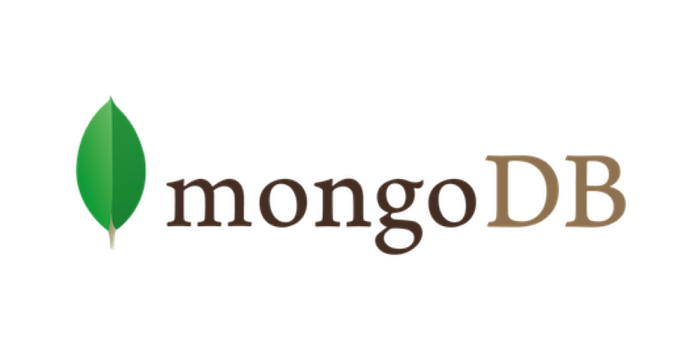
\includegraphics[width=3cm]{img/mongodb}


\subsection{Le SQL}
\begin{itemize}
    \item	\textit{Structured Query Langage} (langage de requêtes structuré).
    \item	Créé en 1974, normalisé en 1986, dernière version parue en 2011.
    \item 	Utilisé par la plupart des SGBD avec de petites différences.
\end{itemize}



\subsection{Exemple de requête}

\footnotesize

\begin{sql}
    \begin{minted}{sql}
SELECT DISTINCT nom, prenom
FROM Auteur
         JOIN Ecrire ON Ecrire.id_auteur = Auteur.id_auteur
         JOIN Livre ON Livre.num_isbn = Ecrire.num_isbn
WHERE Livre.titre LIKE '%s%';
\end{minted}
\end{sql}

\normalsize
Voici comment obtenir la liste des noms et prénoms des auteurs ayant écrit un livre dont le titre comporte la lettre « s». Nous expliquerons comment produire de telles requêtes plus tard.

\subsection{Vocabulaire}
En SQL, les relations s'appellent des \textit{tables}.\\

Les éléments des tables s'appellent des \textit{tuples}.

\subsection{Bilan des termes utilisés}
\begin{center}
    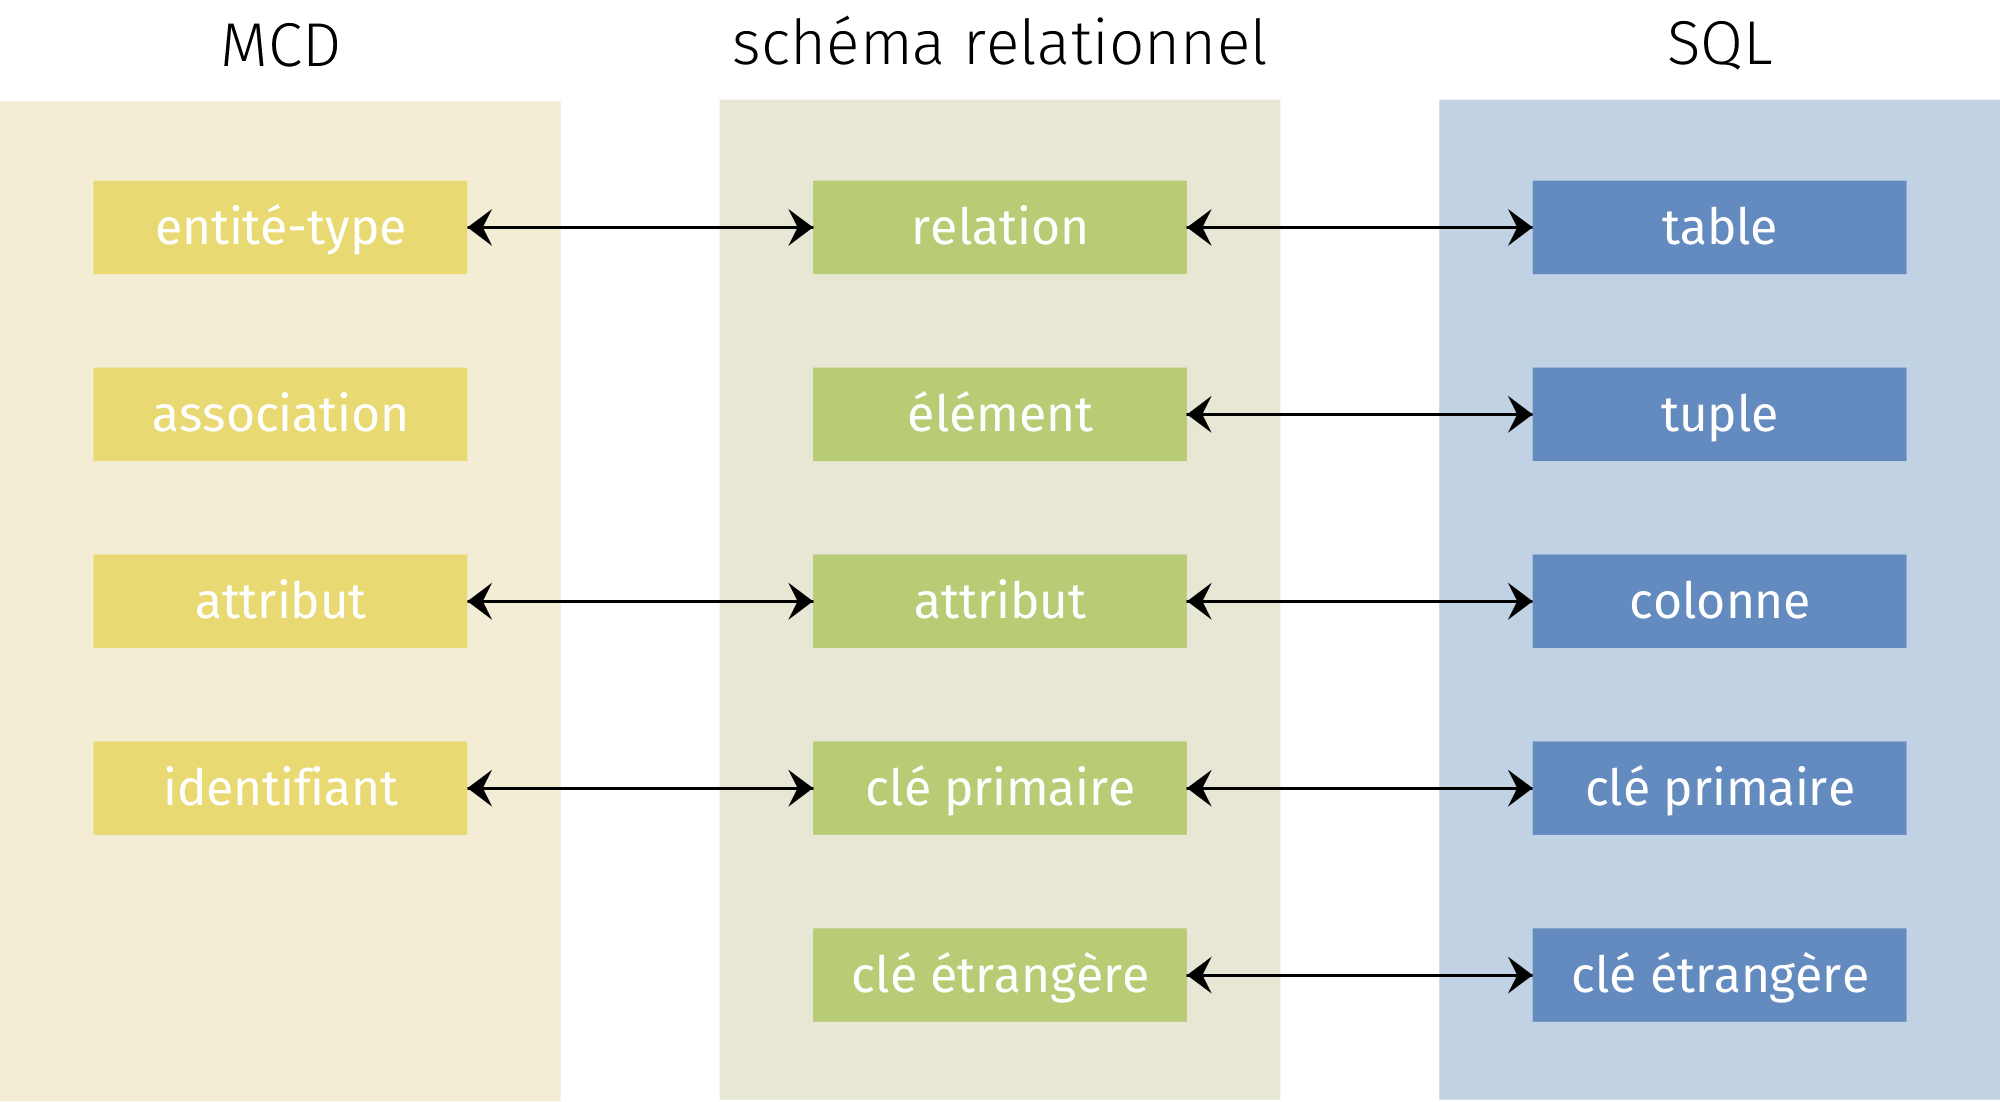
\includegraphics[width=12cm]{img/classification}
\end{center}

\subsection{Conventions}
On écrira les mots-clés SQL en majuscules.\\

On ne met pas d'accents ou d'espaces dans les noms des tables ou des attributs.\\

Les espaces et tabulations n'ont qu'un rôle esthétique.\\

Les requêtes peuvent prendre plusieurs lignes mais doivent se terminer par un point-virgule.\\

On utilisera SQLite car on peut s'en servir avec DB Browser sans installation compliquée.

\section{Création de la BDD}
\subsection{Créer une BDD}

\begin{sql}
    \begin{minted}{sql}
CREATE DATABASE Bibliotheque;
USE Bibliotheque;
\end{minted}
\end{sql}

On n'utilisera pas (ou peu) cette commande dans les exercices.


\subsection{Supprimer une BDD}

\begin{sql}
    \begin{minted}{sql}
DROP DATABASE Bibliotheque;
	\end{minted}
\end{sql}

On n'utilisera pas cette commande non plus.


\subsection{Créer une table}
Voici comment créer la table \textbf{Pays} :

\begin{sql}
    \begin{minted}{sql}
DROP TABLE IF EXISTS Pays; -- recréer la table de zéro
CREATE TABLE Pays
(
    nom_pays   TEXT,
    population INTEGER,
    superficie INTEGER,
    PRIMARY KEY (nom_pays), -- clé primaire
    CHECK (population > 0), -- contraintes utilisateur
    CHECK (superficie > 0)
);
\end{minted}
\end{sql}



\subsection{Table \textbf{Livre}}


\begin{sql}
    \begin{minted}{sql}
DROP TABLE IF EXISTS Livre;
CREATE TABLE Livre
(
    num_isbn INTEGER,
    titre    TEXT,
    annee    TEXT,
    PRIMARY KEY (num_isbn),
    CHECK (date(annee) BETWEEN '1900' AND '2100')
);
\end{minted}
\end{sql}

\mintinline{sql}{date(annee) BETWEEN '1900' AND '2100'} est l'équivalent SQL de\\\mintinline{python}{'1900' <= date(annee) <= '2100'} en Python.

\begin{encadrecolore}{Attention}{UGLiRed}
    SQLite ne connaît pas le type \mintinline{sql}{DATE}, il faut créer des attributs de type \mintinline{sql}{TEXT} et utiliser la fonction \mintinline{sql}{date}. 
\end{encadrecolore}

\subsection{Table \textbf{Livre}}
\begin{sql}
    \begin{minted}{sql}
DROP TABLE IF EXISTS Auteur;
CREATE TABLE Auteur
(
    id_auteur      INTEGER,
    nom_pays       TEXT,
    nom            TEXT,
    prenom         TEXT,
    date_naissance TEXT,
    PRIMARY KEY (id_auteur),
    UNIQUE (nom, prenom), -- contrainte d'unicité
    FOREIGN KEY (nom_pays) REFERENCES Pays (nom_pays)
    /*nom_pays est une clé étrangère*/
        ON DELETE CASCADE
        /*si on supprime des tuples dans Pays, automatiquement
        (en cascade) on supprimera les tuples qui y font
        référence dans Auteur*/
        ON UPDATE CASCADE
        /*si on met à jour les attributs nom_pays dans Pays,
        alors le SGBD les mettra à jour aussi dans Auteur*/
);\end{minted}
\end{sql}

\subsection{Ordre des créations des tables}
On ne peut pas créer \textbf{Auteur} avant d'avoir crée \textbf{Pays} car \textbf{Auteur} possède une clé étrangère liée à \textbf{Pays}.


\subsection{Table \textbf{Ecrire}}
\begin{sql}
    \begin{minted}{sql}
DROP TABLE IF EXISTS Ecrire;
CREATE TABLE Ecrire
(
    id_auteur    INTEGER,
    num_isbn     INTEGER,
    nb_chapitres INTEGER,
    PRIMARY KEY (id_auteur, num_isbn),
    FOREIGN KEY (id_auteur) REFERENCES Auteur (id_auteur)
        ON DELETE CASCADE
        ON UPDATE CASCADE,
    FOREIGN KEY (num_isbn) REFERENCES Livre (num_isbn)
            ON DELETE CASCADE
            ON UPDATE CASCADE
);
\end{minted}
\end{sql}

\section{Variantes syntaxiques et autres}
\subsection{\'Ecriture plus compacte}
On peut signifier qu'un attribut est une clé étrangère dans sa définition même :
\begin{sql}
    \begin{minted}{sql}
DROP TABLE IF EXISTS Ecrire;
CREATE TABLE Ecrire
(
    id_auteur    INTEGER REFERENCES Auteur (id_auteur)
        ON DELETE CASCADE
        ON UPDATE CASCADE,
    num_isbn     INTEGER REFERENCES Livre (num_isbn)
        ON DELETE CASCADE
        ON UPDATE CASCADE,
    nb_chapitres INTEGER,
    PRIMARY KEY (id_auteur, num_isbn)
);
\end{minted}
\end{sql}


\subsection{\'Ecriture plus compacte (bis)}
On peut signifier qu'un attribut est une clé primaire dans sa définition même :
\begin{sql}
    \begin{minted}{sql}
DROP TABLE IF EXISTS Livre;
CREATE TABLE Livre
(
    num_isbn INTEGER PRIMARY KEY,
    titre    TEXT,
    annee    TEXT,
    CHECK (date(annee) BETWEEN '1900' AND '2100')
);
\end{minted}
\end{sql}



\section{Insertion des données dans la BDD}


\subsection{Données de \textbf{Pays}}
\begin{sql}
    \begin{minted}{sql}
INSERT INTO Pays
VALUES ('France', 672051, 67064000),
       ('Italie', 301336, 66436000),
       ('Royaume-Uni', 242900, 60317000);
\end{minted}
\end{sql}
Les attributs des tuples sont dans le même ordre que lors de la création.


\subsection{\textit{Et c\ae tera}}
De même que lors de la création, on ne peut pas insérer de tuples dans \textbf{Auteur} avant d'avoir peuplé \textbf{Pays} : en effet dans un tuple de \textbf{Auteur} tel que \\

\mintinline{sql}{(1, 'France', 'Hugo', 'Victor', '1802-02-26')}\\

Les contraintes de référence font qu'un tuple « France» doit d'abord exister dans \textbf{Pays}.
\section{Exercices}

\begin{exercice}[]
    Ouvrir le fichier \texttt{create\_Auteurs.sql} qui a servi à créer la BDD du cours (avec le bloc-notes ou autre).
    \begin{enumerate}
        \item 	Trouver une écriture compacte telle que vue dans le cours.
        \item 	Trouver une écriture compacte qui n'avait pas été vue.
        \item 	En fouillant « à vue d'\oe il» dans les données
              \begin{enumalph}
                  \item 	Combien y a-t-il de livres ?
                  \item 	Combien y a t-il d'auteurs ?
                  \item 	Où voit-on clairement qu'un auteur a écrit 2 livres ?
              \end{enumalph}
    \end{enumerate}
\end{exercice}
\begin{exercice}[]
    \begin{enumerate}
        \item Voici le modèle relationnel de l'exercice \textbf{Hotel Reservation Client Chambre} du chapitre précédent :\\
              
              \textbf{Hotel}(\uline{nom\_hotel TEXT}, adresse TEXT)\\
              
              \textbf{Chambre}(\uline{num\_ch INTEGER}, prix INTEGER, \dashuline{nom\_hotel TEXT})\\
              
              \textbf{Client}(\uline{num\_client INTEGER}, nom\_client TEXT)\\
              
              
              \textbf{Reservation}(\uline{num\_resa INTEGER}, date\_resa DATE,\dashuline{ num\_client INTEGER},\dashuline{ num\_chambre INTEGER})\\
              
              Écrire le script SQL qui crée cette BDD.
        \item Insérer 3 valeurs de votre choix dans chaque table.
    \end{enumerate}
\end{exercice}
\begin{exercice}[]
    On considère une base de données qui ne contient aucune table.\\
    Dire quelles erreurs produisent les séquences SQL suivantes (tout au moins ce qui n'est pas acceptable du point de vue du cours).
    \begin{enumerate}
        \item 	\begin{minted}{sql}
    DROP TABLE Client;
    CREATE TABLE Client
    (
        cid             INTEGER,
        nom             TEXT,
        prenom          TEXT,
        points_fidelite INTEGER NOT NULL,
            PRIMARY KEY (cid),
        CHECK (points_fidelite >= 0)
    );
        \end{minted}
        \item 	\begin{minted}{sql}
    CREATE TABLE Client
    (
        cid             INTEGER PRIMARY KEY,
        nom             TEXT,
        prenom          TEXT,
        points_fidelite INTEGER NOT NULL,
        CHECK (points_fidelite >= 0)
    );
    CREATE TABLE Commande
    (
        cid  INTEGER PRIMARY KEY, -- variante plus rapide et valide
        pid  INTEGER,
        date TEXT NOT NULL,
        FOREIGN KEY (cid) REFERENCES Client (cid),
        FOREIGN KEY (pid) REFERENCES Client (pid)
    );
    CREATE TABLE Produit
    (
        pid  INTEGER PRIMARY KEY,
        nom  TEXT,
        prix REAL(10, 2) -- 10 chiffres max avant la virgule, 2 après
    );
    \end{minted}
              
        \item \begin{minted}{sql}
    CREATE TABLE Client
    (
        cid             INTEGER PRIMARY KEY,
        nom             TEXT,
        prenom          TEXT,
        points_fidelite INTEGER NOT NULL,
        CHECK (points_fidelite >= 0)
    );
    CREATE TABLE Produit
    (
        pid  INTEGER PRIMARY KEY,
        nom  TEXT,
        prix REAL(10, 2)
    );
    CREATE TABLE Commande
    (
        cid  TEXT REFERENCES Client (cid),
        nomp  INTEGER REFERENCES Produit (nom),
        date TEXT NOT NULL,
        PRIMARY KEY (cid, pid)
    );
    \end{minted}
              
        \item	\begin{minted}{sql}
    CREATE TABLE Client
    (
        cid             INTEGER PRIMARY KEY,
        nom             TEXT,
        prenom          TEXT,
        points_fidelite INTEGER NOT NULL,
        CHECK (points_fidelite >= 0)
    );
    CREATE TABLE Produit
    (
        pid  INTEGER PRIMARY KEY,
        nom  TEXT,
        prix REAL(10, 2)
    );
    CREATE TABLE Commande
    (
        cid  INTEGER,
        pid  INTEGER,
        date TEXT NOT NULL,
        PRIMARY KEY (cid, nomp),
        FOREIGN KEY (cid) REFERENCES Client (cid),
        FOREIGN KEY (pid) REFERENCES Produit (pid)
    );
    
    INSERT INTO Commande VALUES(0, 0, '2020-03-02')
    \end{minted}
    \end{enumerate}
\end{exercice}


\begin{exercice}
    Liste les différents attributs de cette
    relation. Donne le domaine de chaque
    attribut. Pour chaque attribut dire s'il peut jouer ou non le rôle de clef primaire et pourquoi.
    \begin{center}
        \textbf{Film}\\[1em]
        \tabstyle[UGLiOrange]
        \begin{tabular}{|c|c|c|c|c|}
            \hline
            \ccell id & \ccell titre                & \ccell realisateur & \ccell ann\_sortie & \ccell note\_sur\_10 \\
            \hline
            1         & Alien, le huitième passager & Scott             & 1979               & 10                   \\
            2         & Dune                        & Lynch             & 1985               & 5                    \\
            3         & 2001 : l'Odyssée de l'Espace & Kubrick           & 1968               & 9                    \\
            4         & Blade Runner                & Scott             & 1982               & 10                   \\
            \hline
        \end{tabular}\\[2em]
    \end{center}
    
\end{exercice}

\begin{exercice}

    Indique les attributs qui peuvent servir de lien entre ces deux relations.
    
    \begin{center}
        \textbf{Auteur}\\[1em]
        \tabstyle[UGLiOrange]
        \begin{tabular}{|c|c|c|c|c|}
            \hline
            \ccell id & \ccell nom & \ccell prenom & \ccell ann\_naiss & \ccell langue\_ecriture \\
            \hline
            1         & Orwell     & George        & 1903              & anglais                 \\
            2         & Herbert    & Frank         & 1920              & anglais                 \\
            3         & Asimov     & Isaac         & 1920              & anglais                 \\
            4         & Barjavel   & René          & 1911              & français                \\
            5         & Verne      & Jules         & 1828              & français                \\
            ...       & ...        & ...           & ...               & ...                     \\
            \hline
        \end{tabular}\\[2em]
    \end{center}
    
    \begin{center}
        \textbf{Livre}\\[1em]
        
        \begin{tabular}{|c|c|c|c|c|}
            \ccell id & \ccell titre          & \ccell id\_auteur & \ccell ann\_publi & \ccell note \\
            \hline
            ...       & ...                   & ...               & ...               & ...         \\
            34        & La nuit des temps     & 4                 & 1968              & 7           \\
            35        & De la Terre à la Lune & 5                 & 1865              & 10          \\
            36        & Les Robots            & 6                 & 1950              & 9           \\
            ...       & ...                   & ...               & ...               & ...         \\
            \hline
        \end{tabular}\\[2em]
    \end{center}
\end{exercice}

\begin{exercice}
    \begin{enumerate}
        \item 	En partant de la relation \textbf{Film} ci-dessus, crée
              une relation \textbf{Realisateur} (attributs de la
              relation: \texttt{id}, \texttt{nom}, \texttt{prenom} et
              \texttt{ann\_naissance}, tu trouveras toutes les
              informations nécessaires sur le Web).
              Modifie ensuite la relation \textbf{Film} afin d'établir
              un lien entre les relations \textbf{Film} et
              \textbf{Realisateur}. Tu préciseras l'attribut qui
              jouera le rôle de clef étrangère.
              
        \item 	\'Ecris le code \textsc{SQL} permettant de générer les 2 tables.
        \item   \'Ecris le code \textsc{SQL} pour insérer les films et les réalisateurs correspondants.
    \end{enumerate}
\end{exercice}
\chapter{BDD partie 4}
\section{Requêtes SQL}
\subsection{Requête et résultat}
Une requête est une commande SQL et renvoie une table.\\
On se replace dans le contexte du chapitre précédent.

\subsection{Sélection d'attributs}
\begin{minted}{sql}
SELECT nom, prenom
FROM Auteur;
    \end{minted}

\begin{center}
    \tabstyle[UGLiOrange]
    \begin{tabular}{c|c}
        \ccell nom  & \ccell prenom \\
        Ammaniti    & Niccolo       \\
        Avallone    & Silvia        \\
        Camus       & Albert        \\
        Hamilton    & Peter         \\
        Hugo        & Victor        \\
        Murgia      & Michela       \\
        Rhode james & Montague      \\
        Tolkien     & John
    \end{tabular}
\end{center}


\subsection{Sélection de tous les attributs}
\begin{minted}{sql}
SELECT *
FROM Auteur;
    \end{minted}

\begin{center}
    \tabstyle[UGLiOrange]
    \begin{tabular}{c|c|c|c|c}
        \ccell id\_auteur & \ccell nom\_pays & \ccell nom  & \ccell prenom & \ccell date\ naissance \\
        1                 & France           & Hugo        & Victor        & 1802-02-26             \\
        2                 & France           & Camus       & Albert        & 1913-11-07             \\
        4                 & Italie           & Avallone    & Silvia        & 1948-04-13             \\
        5                 & Italie           & Ammaniti    & Niccolo       & 1966-09-25             \\
        6                 & Italie           & Murgia      & Michela       & 1972-06-03             \\
        7                 & Royaume-Uni      & Hamilton    & Peter         & 1960-03-02             \\
        8                 & Royaume-Uni      & Tolkien     & John          & 1892-01-03             \\
        9                 & Royaume-Uni      & Rhode James & Montague      & 1862-08-01
    \end{tabular}
\end{center}


\subsection{Sélection avec condition}
\begin{minted}{sql}
SELECT nom, date_naissance
FROM Auteur
WHERE date(date_naissance) < '1900';
    \end{minted}

\begin{center}
    \tabstyle[UGLiOrange]
    \begin{tabular}{c|c}
        \ccell nom  & \ccell date\_naissance \\
        Hugo        & 1802-02-16             \\
        Tolkien     & 1892-01-03             \\
        Rhode James & 1862-08-01             \\
    \end{tabular}
\end{center}


\subsection{Sélection avec conditions multiples}
\begin{minted}{sql}
SELECT nom, date_naissance
FROM Auteur
WHERE date(date_naissance) < '1900'
  AND nom_pays = 'France';
    \end{minted}

\begin{center}
    \tabstyle[UGLiOrange]
    \begin{tabular}{c|c}
        \ccell nom & \ccell date\_naissance \\
        Hugo       & 1802-02-16             \\
    \end{tabular}
\end{center}


\subsection{Renommer les colonnes}
\begin{minted}{sql}
SELECT titre AS Titre_ouvrage, num_isbn AS Reference_ISBN
FROM Livre
WHERE date(annee) > '2015';
\end{minted}

\begin{center}
    \tabstyle[UGLiOrange]
    \begin{tabular}{c|c}
        \ccell Titre\_ouvrage & \ccell Reference\_ISBN \\
        les misérables        & 9782072730672          \\
        et je t'emmène        & 9782221133651          \\
        d'acier               & 9782867465987          \\
        salvation             & 9791093835334          \\
    \end{tabular}
\end{center}

\subsection{Fonction COUNT}
\begin{minted}{sql}
SELECT COUNT(titre) AS Nb_Livres_avant_2015
FROM Livre
WHERE annee < 2015;    
\end{minted}

\begin{center}
    \tabstyle[UGLiOrange]
    \begin{tabular}{c}
        \ccell Nb\_Livres\_avant\_2015 \\
        4
    \end{tabular}
\end{center}

\subsection{Autres fonctions similaires}
Fonctions MIN, MAX, SUM et AVG (moyenne).

\subsection{\'Eliminer les doublons}
Sans élimination :
\begin{minted}{sql}
SELECT id_auteur
FROM Ecrire;
    \end{minted}

\begin{center}
    \tabstyle[UGLiOrange]
    \begin{tabular}{c}
        \ccell id\_auteur \\
        1                 \\
        1                 \\
        2                 \\
        4                 \\
        5                 \\
        6                 \\
        7                 \\
        8                 \\
        9
    \end{tabular}
\end{center}

Avec élimination :
\begin{minted}{sql}
SELECT DISTINCT id_auteur
FROM Ecrire;
    \end{minted}

\begin{center}
    \tabstyle[UGLiOrange]
    \begin{tabular}{c}
        \ccell id\_auteur \\
        1                 \\
        2                 \\
        4                 \\
        5                 \\
        6                 \\
        7                 \\
        8                 \\
        9
    \end{tabular}
\end{center}
\subsection{Ordonner les tuples}
Ordonner les noms dans l'ordre croissant :
\begin{minted}{sql}
SELECT nom,prenom FROM Auteur
ORDER BY nom ASC;
    \end{minted}

\begin{center}
    \tabstyle[UGLiOrange]
    \begin{tabular}{c|c}
        \ccell nom  & \ccell prenom \\
        Ammaniti    & Niccolo       \\
        Avallone    & Silvia        \\
        Camus       & Albert        \\
        Hamilton    & Peter         \\
        Hugo        & Victor        \\
        Murgia      & Michela       \\
        Rhode james & Montague      \\
        Tolkien     & John
    \end{tabular}
\end{center}
Pour l'ordre décroissant on utilise \mintinline{sql}{DESC}.


\section{Jointures}
\subsection{Principe}
Considérons 2 tables T1 et T2 et supposons que c est une clé étrangère qui fait référence à b.

\begin{center}
    \tabstyle[UGLiOrange]
    \begin{tabular}{c|c}
        \ccell a & \ccell b \\
        0        & 0        \\
        0        & 1        \\
        1        & 1        \\
        2        & 1        \\
        3        & 2        \\
        4        & 5 
    \end{tabular}\hspace{3em}
    \begin{tabular}{c|c}
        \ccell c & \ccell d \\
        0        & 10       \\
        0        & 30       \\
        1        & 12       \\
        2        & 100      \\
        2        & 200 
    \end{tabular}
\end{center}

Voici table qui est la \textit{jointure} T1 et T2 selon la condition b=c :


\begin{center}
    \tabstyle[UGLiOrange]
    \begin{tabular}{c|c|c|c}
        \ccell a & \ccell b & \ccell c & \ccell d \\
        0        & 0        & 0        & 10       \\
        0        & 0        & 0        & 30       \\
        0        & 1        & 1        & 12       \\
        1        & 1        & 1        & 12       \\
        2        & 1        & 1        & 12       \\
        3        & 2        & 2        & 100      \\
        3        & 2        & 2        & 200      \\
    \end{tabular}
\end{center}
C'est la table obtenue en faisant correspondre chaque tuple de T1 avec chaque autre tuple de T2 tel que b et c soient égaux.

\subsection{Applications}
Produire la table des noms des auteurs venant de pays de plus de 61 millions d'habitants :
\begin{minted}{sql}
SELECT nom
from Auteur
         JOIN Pays ON Auteur.nom_pays = Pays.nom_pays
WHERE population > 62000000;
    \end{minted}

\begin{center}
    \tabstyle[UGLiOrange]
    \begin{tabular}{c}
        \ccell nom \\
        Hugo       \\
        Camus      \\
        Avallone   \\
        Ammaniti   \\
        Murgia
    \end{tabular}
\end{center}



Produire la table des noms et prénoms des auteurs ayant écrit un livre dont le titre comporte « la»  :
\begin{minted}{sql}
SELECT DISTINCT nom, prenom
FROM Auteur
         JOIN Ecrire ON Ecrire.id_auteur = Auteur.id_auteur
         JOIN Livre ON Livre.num_isbn = Ecrire.num_isbn
WHERE Livre.titre LIKE '%la%';
\end{minted}

\begin{center}
    \tabstyle[UGLiOrange]
    \begin{tabular}{c|c}
        \ccell nom  & \ccell prenom \\
        Camus       & Albert        \\
        Rodhe James & Montague
    \end{tabular}
\end{center}

\section{Mises à jour}


\subsection{INSERT INTO}
Insérer un nouveau tuple dans la table \textbf{Auteur} :
\begin{minted}{sql}
INSERT INTO Auteur VALUES
    (128,'France','Leleu','Frédéric','1974-05-16');
\end{minted}

Les colonnes doivent être dans le même ordre qu'à la création, sinon utiliser
\begin{minted}{sql}
INSERT INTO Auteur VALUES (nom,id_auteur)
    ('Leleu',128);
\end{minted}

Les colonnes non renseignées prendront par défaut la valeur \mintinline{sql}{NULL} ce qui peut poser problème.


\subsection{DELETE}

Supprimer les tuples de \textbf{Ecrire} dont l'auteur a l'id\_auteur 1:
\begin{minted}{sql}
DELETE FROM Ecrire WHERE id_auteur = 1;
\end{minted}

Penser aux contraintes de références (clé étrangères) : si on supprime un tuple et qu'un tuple d'une autre table fait référence à celui qu'on supprime, cela provoquera une erreur.


\subsection{UPDATE}

Mettre à jour l'id du tuple de \textbf{Auteur} dont le nom est Hugo
\begin{minted}{sql}
UPDATE Auteur
SET id_auteur = 1024
WHERE nom = 'Hugo';
	\end{minted}

Penser aux contraintes de références (clé étrangères) lors de la mise à jour.
\section{Exercices}

\begin{exercice}[ : Prix Nobel]
    \begin{center}
        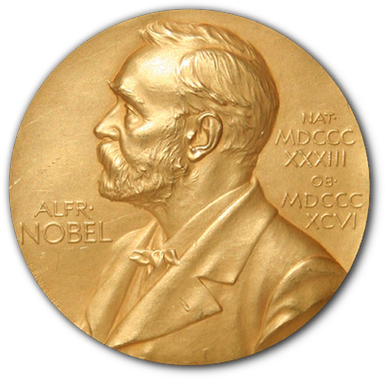
\includegraphics[width=5cm]{img/nobel}
    \end{center}
    \textbf{Premier contact}\\
    
    Avec un éditeur de texte ouvrir le fichier \texttt{create\_nobel.sql}.\\
    En explorant la structure de la base de données, répondez aux questions suivantes :	\\
    \begin{enumerate}
        \item 	Combien de tables possède la base de données ?
        \item 	Combien d'attributs possède la table Nobel ?
        \item 	Quel est le type de l'attribut annee ?\\
    \end{enumerate}
    \textbf{La table Nobel}\\
    
    Importer ce fichier dans DB Browser pour créer la BDD \texttt{nobel.db}.\\
    En explorant les données de la table Nobel, répondez aux questions suivantes :\\
    
    \begin{enumerate}
        \setcounter{enumi}{3}
        \item 	Combien d'enregistrements possède la table Nobel ?
        \item 	Dans quelle discipline Paul Krugman est-il devenu Prix Nobel ?
        \item 	En quelle année Albert Fert a-t-il eu le prix Nobel ?	\\
    \end{enumerate}
    
    \textbf{Requêtes d'interrogation}\\
    
    En utilisant l'onglet : « Exécuter le SQL », indiquez le code SQL permettant de répondre aux questions suivantes :\\
    
    \begin{enumerate}
        \setcounter{enumi}{6}
        \item  Comment afficher le nom de tous les lauréats en évitant les doublons ? (809 enregistrements)
        \item Comment afficher le nom de toutes les disciplines en évitant les doublons ? (6 enregistrements)
        \item  Quelle est la discipline de Wilhelm Conrad Röntgen ? (1 enregistrement)
        \item  Dans quelle discipline Paul Krugman est-il devenu Prix Nobel ? (1 enregistrement)
        \item  En quelle année Albert Fert a-t-il eu le prix Nobel ? (1 enregistrement)
        \item  Quelle est l'année de distinction de Pierre Curie ? (1 enregistrement)
        \item  Quelle est l'année de distinction et la matière de Bertha von Suttner ? (1 enregistrement)
        \item  Quels sont les lauréats distingués au XXI e siècle ? (97 enregistrements)
        \item  Quels sont les lauréats du prix Nobel de la Paix durant la deuxième guerre mondiale ? (2 enregistrements)
        \item  Quels sont les lauréats distingués en Médecine en 1901 et en 2001 ? (4 enregistrements)
        \item  Quels sont les lauréats des prix Nobel de Physique et de Médecine en 2008 ? (3 enregistrements)	\\
    \end{enumerate}
    
    \textbf{Requêtes d'agrégation}\\
    
    \begin{enumerate}
        \setcounter{enumi}{17}
        \item  Combien d'enregistrements au total comporte la table ? (816 enregistrements)
        \item  Combien de personnes ont reçu le prix Nobel de la paix ? (119 enregistrements)
        \item  Combien de personnes ont reçu le prix Nobel de littérature ? (105 enregistrements)
        \item  Combien de personnes ont reçu le prix Nobel de mathématiques ? (0 enregistrements)
        \item  Combien de personnes ont reçu un prix Nobel en 1901 ? (6 enregistrements)
        \item  Combien de personnes ont reçu un prix Nobel de chimie en 1939 ? (2 enregistrements)
        \item  En quelle année a été décerné le premier prix Nobel d'économie ? (Réponse : 1969)
        \item  Combien de prix Nobel a reçu Marie Curie ? (Réponse : 2)
        \item  Quels sont les prix lauréats, leur discipline et l'année de distinction de tous les prix Nobel contenant Cohen dans leur nom (on ne fera pas de distinction de casse) ? (2 enregistrements)
        \item  Combien y a-t-il eu de lauréats en Physique et en Chimie ? (335 enregistrements)
        \item  Combien y a-t-il eu de lauréats de Médecine et de littérature en 2000 ? (4 enregistrements)
        \item  Nombre de lauréats différents parmi les prix Nobel de la paix ? (116 enregistrements)\\
    \end{enumerate}
    
    \textbf{Requêtes de mise à jour}\\
    \setcounter{enumi}{29}
    En utilisant l'onglet Exécuter le SQL, indiquez le code SQL permettant de répondre aux questions suivantes :\\
    
    \begin{enumerate}
        \item En 2019, Esther Duflo a reçu le prix Nobel d'économie. Écrivez la requête permettant d'insérer cet enregistrement.
        \item  Quelle requête permet de modifier l'enregistrement précédent pour accoler le nom d'époux (Banerjee) après celui de Duflo ?
        \item   De nombreuses pétitions circulent pour retirer le prix Nobel à Aung San Suu Kyi. Quelle requête permettrait cela ?
    \end{enumerate}
\end{exercice}






\begin{exercice}[ : JO]
    Nous allons travailler sur une base de données liée aux Jeux Olympiques de Londres qui ont eu lieu en 2012.\\
    \begin{center}
        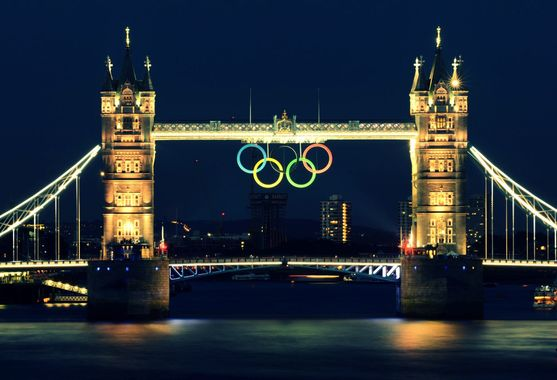
\includegraphics[width=8cm]{img/jo_london}
    \end{center}
    
    \textbf{\large Partie 1 : \'Etude du schéma relationnel}\\
    
    Avec un éditeur de texte tout simple, ouvrir le fichier \texttt{create\_JO.sql}, regarder les lignes qui définissent les différentes tables de la BDD et donner sous forme écrite son schéma relationnel en soulignant clés primaires (en trait plein) et clés étrangère (en pointillés).\\
    
    \textbf{\large Partie 2 : Requêtes SQL}\\
    
    Avant toute chose, ouvrir DB Browser, importer le fichier \texttt{create\_JO.sql} pour créer la BDD \texttt{JO.db}.\\
    Ensuite exécuter les bonnes requêtes SQL pour obtenir les données suivantes.\\
    
    \textbf{Requêtes sans jointures}
    \begin{enumerate}
        \item 	Afficher le nom et prénom des sportifs. Combien y en a-t-il ?
        \item 	Afficher les codes des pays dont viennent les sportifs par ordre alphabétique en éliminant les doublons.
        \item 	Afficher la liste des sportifs français (utiliser cio = 'France').
        \item 	Afficher la liste des 301 disciplines triées par l'identifiant du sport auxquelles elles se rapportent.
        \item 	Afficher les noms des 86 pays situés après la France et avant la Russie (Russia) par ordre alphabétique.\\
              Utiliser les opérateurs inférieur et supérieur. Remarquer que l'opérateur \mintinline{SQL}{BETWEEN} ne produit pas le résultat attendu (88 pays).
        \item 	Afficher les 98 identifiants de discipline dont au moins une épreuve a eu lieu entre le 27 et le 31 juillet 2012 inclus.
        \item 	Afficher les noms des 61 sportifs qui sont soit français (FRA) soit britanniques (GBR).
        \item 	Afficher les intitulés des 131 disciplines contenant la chaîne de caractères «WOMEN».
              
        \item  Donner les 3 pays (CIO, nom) dont on ne connaît pas le code ISO2 ou ISO3 (utiliser le critère \mintinline{sql}{IS NULL}).
        \item 	Donner les noms et prénoms des 2 sportifs dont le sexe est mentionné dans la BDD.
        \item  	À l'aide de la fonction \mintinline{sql}{COUNT}, donner le nombre de sports (pas la liste).
        \item  Donner le nombre de discipline(s) du sport d'identifiant 1 (pas la liste).
              
              
        \item Combien de noms de familles différents sont portés par les sportifs ?
        \item Donner le nombre de pays n'ont pas d'ISO2.
        \item Donner le nombre de médailles d'or attribués lors de ces JO.
        \item Afficher en une table le premier et le dernier évènement sportif	de ces JO.\\
    \end{enumerate}
    \textbf{Requêtes avec jointures}
    \begin{enumerate}
        \setcounter{enumi}{16}
        \item Afficher la listes des noms et prénoms des sportifs européens.
        \item Afficher la liste des disciplines dépendant de l'athlétisme.
        \item Afficher toutes jours pendant lesquels un évènement lié à l'athlétisme eu lieu.
        \item Afficher les noms, prénoms et médailles gagnées par des sportifs dont le sexe figure dans la BDD.
        \item Afficher la liste des Français médaillés d'or.
        \item Afficher les noms, prénoms, sports et disciplines des sportifs ayant obtenu une médaille d'or.
    \end{enumerate}
    
\end{exercice}
\end{document}